% TEMPLATE for Usenix papers, specifically to meet requirements of
%  USENIX '05
% originally a template for producing IEEE-format articles using LaTeX.
%   written by Matthew Ward, CS Department, Worcester Polytechnic Institute.
% adapted by David Beazley for his excellent SWIG paper in Proceedings,
%   Tcl 96
% turned into a smartass generic template by De Clarke, with thanks to
%   both the above pioneers
% use at your own risk.  Complaints to /dev/null.
% make it two column with no page numbering, default is 10 point

% Munged by Fred Douglis <douglis@research.att.com> 10/97 to separate
% the .sty file from the LaTeX source template, so that people can
% more easily include the .sty file into an existing document.  Also
% changed to more closely follow the style guidelines as represented
% by the Word sample file. 

% Note that since 2010, USENIX does not require endnotes. If you want
% foot of page notes, don't include the endnotes package in the 
% usepackage command, below.

% This version uses the latex2e styles, not the very ancient 2.09 stuff.
\documentclass[letterpaper,twocolumn,10pt]{article}
%\usepackage{usenix,epsfig,endnotes}
\usepackage{usenix}
\usepackage{epsfig}
\usepackage{comment}
%\usepackage{subfigure}
\usepackage[pdftex]{color}
\usepackage{url}
\usepackage{listings}
\usepackage{textcomp}
\usepackage{gnuplot-lua-tikz}
\usepackage{amssymb}
\usepackage{amsmath}
\usepackage{minted}
\usepackage{bm}
\usepackage{paralist}
\usepackage{ulem}
\usepackage{subcaption}
\usepackage{algorithm}
\usepackage{algpseudocode}
\usepackage{graphicx}
\definecolor{lbcolor}{rgb}{0.9,0.9,0.9}

\lstset{
	backgroundcolor=\color{lbcolor},
		tabsize=4,
		rulecolor=,
		language=matlab,
		basicstyle=\scriptsize,
		upquote=true,
		aboveskip={1.5\baselineskip},
		columns=fixed,
		showstringspaces=false,
		extendedchars=true,
		breaklines=true,
		prebreak = \raisebox{0ex}[0ex][0ex]{\ensuremath{\hookleftarrow}},
		frame=single,
		showtabs=false,
		showspaces=false,
		showstringspaces=false,
		identifierstyle=\ttfamily,
		keywordstyle=\color[rgb]{0,0,1},
		commentstyle=\color[rgb]{0.133,0.545,0.133},
		stringstyle=\color[rgb]{0.627,0.126,0.941},
}


\newcommand{\rb}[1]{{\color{red}{\it RB: #1}}}
\newcommand{\dz}[1]{{\color{blue}{\it DZ: #1}}}
\newcommand{\dm}[1]{{\color{green}{\it DM: #1}}}
\newcommand{\jv}[1]{{\color{orange}{\it JV: #1}}}

\newlength{\saveparindent}
\setlength{\saveparindent}{\parindent}
\newlength{\saveparskip}
\setlength{\saveparskip}{\parskip}

\newenvironment{newenumerate}{%
\begin{list}{({\rm \arabic{ctr}})\hfill}{\usecounter{ctr}\labelwidth=17pt%
\labelsep=6pt \leftmargin=23pt \topsep=.5pt%
\setlength{\listparindent}{\saveparindent}%
\setlength{\parsep}{\saveparskip}%
\setlength{\itemsep}{5pt} }}{\end{list}}

\newenvironment{newitemize}{%
\begin{list}{\hspace{3pt}$\bullet$\hfill}{\labelwidth=12pt%
\labelsep=3pt \leftmargin=15pt \topsep=1pt%
\setlength{\listparindent}{\saveparindent}%
\setlength{\parsep}{\saveparskip}%
\setlength{\itemsep}{1pt}}}{\end{list}}

\begin{document}

%don't want date printed
\date{}

%make title bold and 14 pt font (Latex default is non-bold, 16 pt)
\title{Large-scale data mining with generalized matrix operations}

%for single author (just remove % characters)
%\author{
%{\rm Da Zheng, Randal Burns}\\
%Department of Computer Science \\
%Johns Hopkins University
%\and
%{\rm Joshua Vogelstein}\\
%Institute for Computational Medicine \\
%Department of Biomedical Engineering \\
%Johns Hopkins University
% copy the following lines to add more authors
%\and
%{\rm Alexander S. Szalay}\\
%Department of Physics and Astronomy \\
%Johns Hopkins University
%} % end author

\maketitle

% Use the following at camera-ready time to suppress page numbers.
% Comment it out when you first submit the paper for review.
\thispagestyle{empty}


\subsection*{Abstract}

\section{Introduction}
% What problem are you going to solve.

The explosion of data volume and the increasing complexity of data analysis
generate a growing demand for scalable statistical analysis and machine
learning tools that are simple and efficient.
Simple tools need to be programmable, interactive, and extensible, 
allowing scientists to encode and deploy complex algorithms. 
Successful examples include R, SciPy, and Matlab.  Efficiency dictates that
tools should leverage modern computer architectures, including scalable
parallelism, high-speed networking, and fast I/O from memory and solid-state
storage. Unfortunately, the current approach for taking advantage of the full
capacity of modern parallel systems often uses a low-level programming
language such as C or FORTRAN and parallelizes computation with MPI or OpenMP.
This approach is time-consuming and error-prone, and requires machine learning
researchers to have expert knowledge in the parallel programming models.
 
% How have others addressed the problem?

While conventional wisdom addresses large-scale data analysis with clusters
\cite{mapreduce,spark,h2o,systemml,tensorflow,petuum}, recent works
\cite{flashgraph,gridgraph,Matveev17,hotos} demonstrate a single-machine solution
can deal with large-scale data analysis problems efficiently in a multicore
machine. The advance of solid-state drives (SSDs) creates new opportunities
for a single-machine solution to tackle data analysis efficiently at a larger scale
with a cheaper price. SSD-based graph analysis frameworks \cite{flashgraph, gridgraph}
have demonstrated the comparable efficiency to state-of-the-art in-memory graph
analysis, while scaling to arbitrarily large datasets. This work extends
these findings to matrix operations using SSDs. Matrices are the most prevalent
and intuitive representation for machine learning and data analysis tasks.
\dz{we need to say more about the advantage of a single-machine solution
compare with cluster solutions.}

% Why is it hard?

% What is the nature of your solution?
To provide a simple programming language for efficient and scalable machine
learning, we present FlashR, an interactive R-based programming framework that
executes R code in parallel and
out of core automatically for large-scale data analysis. FlashR stores large
vectors and matrices on SSDs and overrides many R functions in the R
\textit{base} package for these external-memory vectors and matrices.
As such, FlashR executes existing R code without or with little modification.
FlashR focuses on optimizations in a single machine (with multiple CPUs and
many cores) and scales matrix operations beyond memory capacity by 
utilizing solid-state drives (SSDs).  
%This paper does not address distributed matrix operations, but, 
%FlashR is suitable for executing the local part of a distributed 
%computation.   
Our evaluation shows that we can solve billion row, Internet-scale 
problems on a single thick node, which can prevent the complexity,
expense, and power consumption of distributed systems when they are
not strictly necessary \cite{hotos}.

%These machines typically have multiple processors with many CPU cores and
%a large amount of memory. They are also equipped with fast flash
%memory such as solid-state drives (SSDs) to further extend memory capacity.
%This conforms to the node design for supercomputers \cite{Ang14}.

% Why is it new/different/special?

To utilize the full capacity of a large parallel machine, we need to overcome
many technical challenges to move data from SSDs to CPU efficiently for matrix
computations,
notably the large performance disparities between CPU and memory and between
memory and SSDs. The ``memory gap'' \cite{Wilkes01} continues to grow, with 
the difference between CPU and DRAM performance increasing exponentially. 
There are also performance differences between
local and remote memory in a non-uniform memory architecture (NUMA), which are prevalent
in modern multiprocessor machines. 
RAM outperforms SSDs by an order of magnitude for both latency and throughput.
%Even though the I/O
%performance of SSDs has advanced to outperform hard drives by a large factor,
%FDespite advances in SSD I/O performance, 
%they remain an order of magnitude slower than RAM.
%Most matrix computation engines increase data movement,
%because they perform an operation on an entire input matrix prior to moving 
%to the next operation.
% RB -- 
%On the other hand, many analysis tasks are
%data-intensive. Matrix
%formulation further increases data movement between CPU and SSDs because
%a matrix computation framework typically performs an operation
%on the entire input matrices before moving to the next operation.
% As such,
%the performance of the data analysis tasks is usually limited by memory
%bandwidth instead of computing power.

FlashR evaluates expressions lazily and fuses operations aggressively
in a single parallel execution job to minimize data movement. FlashR
builds a directed acyclic graph (DAG) to represent a sequence of matrix
operations and grows a DAG as much as possible to increase the ratio of
computation to I/O. When evaluating the computation in a DAG, FlashR
performs two levels of matrix partitioning to reduce data movement in
the memory hierarchy. FlashR by default materializes
only the output matrices (leaf nodes) of a DAG and keeps materialized results in
memory in order to minimize data written to SSDs. FlashR streams
data from SSDs to maximize I/O throughput for most computation tasks.

% What are it's key features?

We implement multiple machine learning algorithms, including principal component
analysis, logistic regression and k-means, in FlashR. On a large parallel machine
with 48 CPU cores and fast SSDs, the out-of-core execution of these R implementations
achieves performance comparable to in-memory execution, while significantly
outperforming the same algorithms in H2O \cite{h2o} and Spark MLlib
\cite{spark}. FlashR effortlessly scales to datasets with billions
of data points and its out-of-core execution uses a negligible amount of memory
compared with the dataset size. In addition, FlashR executes the R functions
in the R MASS \cite{mass} package with little modification and outperforms
the execution of the same functions in Revolution R Open \cite{rro} by more
than an order of magnitude.

We believe that FlashR significantly lowers the requirements for writing
parallel and scalable implementations of machine learning algorithms; it also
offers new
design possibilities for data analysis clusters, replacing memory with larger
and cheaper SSDs and processing bigger problems on fewer nodes.
FlashR is released as an open-source project at http://flashx.io/.


\section{Related Work}
BLAS

Array-oriented programming languages such as APL


\section{Design}

FlashMatrix is a general-purpose data analysis framework that provides
matrix-oriented programming interface. The architecture of FlashMatrix
is shown in Figure \ref{fig:arch}. It provides a very small set of
generalized vector and matrix operators and implements a large number of
vector and matrix operators in R with the generalized operators. The generalized
operators can be executed on each of the data containers supported by
FlashMatrix. The optimizer in FlashMatrix merges multiple operators to
reduce I/O access and achieve better parallelization.

FlashMatrix stores large data containers on SSDs through SAFS \cite{safs},
a user-space filesystem for a large SSD array, to fully utilize high I/O
throughput of the SSDs. For most of the operations, FlashMatrix accesses
data in a data container sequentially to maximize I/O throughput of SSDs.
FlashMatrix keeps some of the large data containers in memory to effectively
utilize memory in a large-RAM machine.

\begin{figure}
\centering
\includegraphics[scale=0.3]{./architecture.pdf}
\caption{The architecture of FlashMatrix.}
\label{fig:arch}
\end{figure}

\subsection{SAFS}

SAFS \cite{safs} is a user-space filesystem for a high-speed SSD array in
a NUMA (non-uniform memory architecture) machine. It is implemented as
a library and runs in the address space
of its application. It is deployed on top of the Linux native filesystem.
SAFS was originally designed for optimizing small I/O accesses. However,
sparse matrix multiplication and dense matrix operations
generate much fewer but much larger I/O. Therefore, we provide additional
optimizations to maximize sequential I/O throughput from a large SSD array.

The original SAFS has a dedicated I/O thread for each SSD. The I/O thread
accesses the SSD exclusively to avoid lock contention in the Linux kernel.
Application threads have to send I/O requests to one of the I/O threads
with message passing when accessing data from SSDs. It is necessary to have
one I/O thread for
an SSD when applications issue many small I/O accesses because processing
a large number of I/O accesses consumes a significant number of CPU cycles.
However, when the workload only has large I/O requests, each I/O request takes
much longer time to complete. As a result, the I/O threads are constantly put
into sleep while waiting for I/O and each I/O completion may suffer from
the latency of a thread context switch.

The latency of a thread context switch becomes noticeable on a high-speed SSD
array under a sequential I/O workload and it becomes critical to avoid thread
context switch to gain I/O performance. Therefore, instead of having an I/O
thread for each SSD, we use only a single I/O thread for each NUMA node, which
is responsible for all of the SSDs connected to the NUMA node. As such, an I/O
thread processes many more I/O requests to amortize the latency of a context
switch. Similarly, application threads communicate with I/O threads through
message passing when issuing I/O requests. If the computation in application
threads did not saturate CPU, SAFS would put the application threads into
sleep while they were waiting for I/O. This results in many thread context
switches and underutilization of both CPU and SSDs. To saturate I/O,
an application thread issues asynchronous I/O and poll for I/O to avoid thread
context switches after completing all computation available to it.

To better support access to many relatively small files simultaneously, SAFS
stripes data in a file across SSDs with a different striping order for each file.
This strategy stores data from multiple files evenly across SSDs and improves
I/O utialization. Due to the sequential I/O workload, FlashEigen stripes data
across SSDs with a large block size, on the order of megabytes, to increase I/O
throughput and potentially reduce write amplification on SSDs \cite{Tang15}.
Such a large block size may cause storage skew for small files
on a large SSD array if every file stripes data in the same order. Using
the same striping order for all files may also cause skew in I/O access.
Therefore, SAFS generates a random striping order for each file to evenly
distribute I/O among SSDs when a file is created. SAFS stores the striping
order with the file for future data retrieval.

\subsection{Data containers}
FlashMatrix supports both dense matrices and sparse matrices. FlashMatrix
represents a vector as a dense matrix. In this work, we mainly focus on
dense matrices. Some dense matrices are physically stored in memory or on SSDs,
but some are stored virtually. All elements in a matrix have the same primitive
type and FlashMatrix supports all primitive types in C/C++.
All matrices in FlashMatrix are immutable, which is required by lazy evaluation.
Each matrix has two identifiers: one for the matrix itself and the other for
the data in the matrix. When a matrix is cloned or transposed, the two matrices
have different matrix Ids but share the same matrix data Id.

\subsubsection{Tall-and-skinny matrix} \label{sec:tas_mat}

Tall-and-skinny (TAS) dense matrices commonly exist in many data mining
algorithms. As suggested by the name, these matrices have one of the dimensions
much larger than the other dimension (Figure \ref{fig:tas_mat}). A vector is
a special case of such a matrix. Many data matrices contain a large set of
data points with a relatively small number of features, so the shape of
the data matrices is usually tall and skinny. FlashMatrix can store TAS
matrices in memory and on SSDs and optimizes matrix operations specifically
for these matrices.

There also exist many wide-and-narrow matrices. For simplicity, we also refer
to wide-and-narrow matrices as a TAS matrix. 

\begin{figure}
	\centering
	\includegraphics[scale=0.5]{./dense_matrix.pdf}
	\caption{The format of a tall-and-skinny dense matrix.}
	\label{fig:tas_mat}
\end{figure}

For parallelization and efficient data access, TAS matrices are partitioned
horizontally and in multiple levels (Figure \ref{fig:tas_mat}).
\begin{itemize}
\item NUMA-level partitioning: When a TAS
matrix is stored in memory, it is partitioned across NUMA nodes to achieve
data locality and fully utilize memory bandwidth. NUMA-level partitioning
tries to map partitions of different vectors/matrices involved in computation
to the same NUMA node to reduce inter-processor communication. As such,
the partition size (the number of rows in a partition) is a global parameter
and is not affected by the number of columns in a matrix. Having NUMA-level
partitioning helps us scale computation to a cluster.
\item I/O-level partitioning: Both in-memory and external-memory matrices have
I/O-level partitioning. A worker thread gets an I/O-level partition from each
matrix for computation and the partition size needs to be relatively large
(in the order of megabytes) to reduce overhead of retrieving a partition from
a matrix. The number of rows in an I/O-level partition is determined locally
and can be affected by the number of columns in a matrix.
All elements in an I/O-level partition are stored contiguously.
For an external-memory matrix, the I/O-level partition size determines an I/O
size. For an in-memory matrix, the partition size determines the size of
contiguous memory required in memory allocation (see Section \ref{sec:mem}).
\item CPU-level partitioning: We further split a matrix into smaller partitions
to reducing CPU cache misses when evaluating a sequence of matrix operations
(Section \ref{sec:lazy_eval}). For this level of partitioning, we keep
a partition small enough (in the order of kilobytes) to fit in CPU L1 cache.
The number of rows in a CPU-level partition is determined at runtime and
is affected by the number of columns in a matrix.
\end{itemize}
The number of rows in each level of partitioning is $2^i$

FlashMatrix supports both row-major and column-major matrices to avoid physical
data copy for some matrix operations such as matrix transpose. Due to
the partitioning scheme shown above, a column in a column-major TAS matrix
is not stored contiguously. FlashMatrix optimizes matrix operations for both
data layouts. The layout of a matrix is generally
determined by a FlashMatrix operation but can also be determined by users. 

If a dense matrix is stored on SSDs, it is stored in an SAFS file and we rely
on SAFS to stripe data across SSDs. SAFS stripes data in a file across SSDs
with a different striping order for each file.
This strategy stores data from multiple files evenly across SSDs and improves
I/O utilization. Due to the sequential I/O workload, FlashEigen stripes data
across SSDs with a large block size, on the order of megabytes, to increase I/O
throughput and potentially reduce write amplification on SSDs \cite{Tang15}.
Such a large block size may cause storage skew for small files
on a large SSD array if every file stripes data in the same order. Using
the same striping order for all files may also cause skew in I/O access.
Therefore, SAFS generates a random striping order for each file to evenly
distribute I/O among SSDs when a file is created. SAFS stores the striping
order with the file for future data retrieval.

\subsubsection{Virtual matrix} \label{virt_mat}
There are many cases that we do not need to store data of a matrix physically.
Instead, we use a special matrix that stores computation along with the input
of the computation, which we refer to as \textit{virtual matrix}. When a
\textit{virtual matrices} is used in computation, its data is generated on
the fly. A simple example is a matrix with all elements having the same value.
We never need to allocate memory for such a matrix physically.

\textit{Virtual matrices} becomes very useful in lazy evaluation (in Section
\ref{lazy_eval}).


With lazy evaluation, an operator outputs a special matrix to represent
the operation result and this special matrix does not store the actual data of
the operation result. Instead, it stores the computation and a reference to
the input matrices. We refer to these special matrices as
\textit{virtual matrices}.

\subsubsection{A group of dense matrices}
In some applications, we construct a group of dense matrices and always perform
operations on them together.

%\subsection{Basic operations} \label{sec:basic}
%create a data container

%data container conversion

%matrix operations: convert data layout and transpose.

%append an element to a vector can be implemented as physically appending the element
%to the vector. The result vector becomes the new vector, and the original vector
%becomes the sub-vector of the new vector.

\subsection{Generalized computation operations} \label{sec:generalized}
To enhance the flexibility and simplify the implementation, FlashMatrix only
provides a small set of generalized operators on vectors and matrices.
The current implementation has four generalized operators: \textit{inner product},
\textit{apply}, \textit{aggregation} and \textit{groupby}. Each operator
accepts user-defined functions (UDF). Like most of R functions, these operators
do not change data in the input data containers and each operation generates
a new data container.

FlashMatrix does not allow to access users to access individual elements.

\textit{Inner product} is a generalized matrix multiplication. It replaces
multiplication and addition in matrix multiplication with two user-defined
functions, respectively. As such, we can define many operations with inner
product. For example, we can use inner product to compute various pair-wise
distance matrics of vectors such as Euclidean distance \cite{euclidean} and
Hamming distance \cite{hamming}. We can also apply inner product to sparse
matrices to compute PageRank, belief propagation, etc.
Even though we can implement matrix multiplication with inner product,
FlashMatrix still relies on BLAS to implement matrix multiplicatoin for
float-point matrices to achieve speed and float-point precision required by
many numeric libraries such as the Trilinos eigensolver \cite{anasazi}.

\textit{Apply} is a generalized form of element-wise operations and has
multiple variants. The simplest form of \textit{apply}, denoted with
\textit{sapply}, is a generalized element-wise unary operation whose
UDF takes an element in a vector or a matrix at a time and outputs a value.
We can use it to implement unary operations such as negation, square root
or type casting of individual elements in a vector or a matrix. The second
form of \textit{apply}, denoted with \textit{mapply2}, is a generalized
element-wise binary operation whose UDF takes an element from each vector
or matrix and outputs a single value. We use it to implement many binary
matrix operations such as matrix addition and subtraction. The third form of
\textit{apply}, denoted by \textit{apply\_mat}, is a generalized row-wise or
column-wise operation whose UDF takes a row or a column at time and outputs
a vector of elements.

\textit{Aggregation} takes multiple elements and outputs a single element.
It has two forms on matrices. The first form, denoted by \textit{agg\_arr}
aggregates over all elements on a matrix. Operations such as summation and
maximum are special cases of the first form. The second form, denoted by
\textit{agg\_mat} aggregates over each individual row or column.
Row sum and column sum are special cases of the second form.

\textit{Groupby} takes a vector of elements along with a vector of categorical
values and invokes UDF on the elements associated with the same categorical
value. \textit{Groupby} also works on a matrix if we view a matrix as a vector
of vectors.

The function of some of the operators overlaps. For example, \textit{apply\_mat}
is a generalized form of \textit{agg\_mat}, but \textit{agg\_mat} can be
implemented more efficiently. Therefore, FlashMatrix provides both operators.

\subsection{Vectorized user-defined function}
UDF potentially introduces significant computation overhead. Traditionally,
UDF is applied to every individual element in a data container and, thus,
the computation on every element suffers from the large overhead of a function
call. Therefore, relying on UDF to implement commonly used vector and matrix
operations reduces the performance of the entire system significantly.
We need to highly optimize UDF to achieve the same performance as
the specialized matrix operations.

To amortize the overhead of function calls, all generalized operators take
vectorized user-defined functions (VUDF), which operates on an array of elements
instead of individual elements. The number of elements in an invocation of
VUDF determines how much overhead is amortized. However, too many elements
in one invocation potentially increase CPU cache misses when the computation
is constructed in a DAG shown in Section {}. For the elements of primitive
types, the number of elements in one invocation of VUDF can be as large as 1000,
which can still perfectly fit in the L1 CPU cache.

The generalized operators require multiple forms of VUDF. The first form takes
two arrays with the same number of elements and outputs an array of the same
length as the input arrays. The second form takes one array of elements and
a single element and outputs an array of the same length as the input array.
The first two forms are essential for binary operations such as
\textit{inner product} and \textit{mapply2} as well as \textit{agg\_mat} and
\textit{groupby\_mat}.
The third form takes an array of elements and outputs an array of the same
length, which is essential for \textit{sapply}.
The fourth form takes an array of elements and outputs a single element,
which is essential for \textit{aggregation}.

FlashMatrix has many commonly used VUDFs implemented in the framework by default.
These VUDFs wrap basic operations built in many programming languages and
libraries. For example, FlashMatrix provides arithmetic operations such as addition
and subtraction, relational operations such as equal to and less than, logical
operations such as logical AND and logical OR, as well as commonly used
math functions such as computing absolute values and square root. FlashMatrix
also provides a set of VUDFs to cast primitive element types. The built-in
binary operation usually needs to support three forms: form1, form2 and form3,
while the unary operation only needs to support form3. In addition, built-in
VUDFs also need to support different element types. Thus, each basic operation
supported by FlashMatrix has multiple VUDF implementations.

To reduce the number of VUDF implementations for different element types, form1
and form2 require the input elements to have the same type. If a generalized
operator gets two data containers with different element types, it first casts
the type of the elements in one container to match the element type of the other
container. Type casting follows the usual arithmetic conversions \cite{}
commonly seen in many programming languages. The type casting is performed
laziy and no additional data container is generated in type casting
(in Section \ref{sec:lazy_eval}).

For easier parallelization, generalized operators assume that VUDF is stateless.
Therefore, the generalized operators carry the mutable state of the computation.
However, VUDF can carry immutable values to simplify some implementations.

All different kinds of vectorized operators such as scatter and gather, aggregation.

We can use the basic VUDF to construct more complex VUDF for other generalized operators.


\subsection{Lazy evaluation} \label{sec:lazy_eval}
It is expensive to perform each matrix operation individually when matrices
become large. It causes significant I/O for
external-memory matrices and considerable memory allocation overhead for
in-memory matrices. Instead, FlashMatrix evaluates matrix operations lazily
and postpones evaluation whenever possible and uses a \textit{virtual matrix}
(in Section \ref{virt_mat}) to represent the output of a matrix operation.

There are multiple benefits with lazy evaluation. For external-memory matrices,
it reduces I/O, especially writes to SSDs. It is beneficial for in-memory
matrices because because it is expensive to allocate large memory chunks.
Another benefit is to enable operation fusion to improve parallelization
\cite{Ching12}. By taking special care of data movement in fused operations,
we minimize data movement between memory and CPU cache and achieve performance
close to manually-written C code.

The current implementation of FlashMatrix applies lazy evaluation to most of
the generalized operators. Lazy evaluation can be easily applied to
\textit{sapply} and \textit{mapply} because these two operations element-wise
operations. We also apply lazy evaluation to \textit{apply\_mat} and
\textit{agg\_mat} when these two operators runs on rows of a TAS matrix.
It is also applied to \textit{inner product} when \textit{inner product} runs
on a TAS matrix and a small matrix. In general, lazy evaluation is applied to
any generalized operator that outputs a large matrix.

To enable lazy evaluation, all matrices in FlashMatrix are immutable.
As such, \textit{virtual matrices} can generate the same result every time
they are materialized. As such, every matrix operation generates a new matrix
and a matrix is garbage collected when there are not any references to it.

\subsection{Matrix materialization}
Lazy evaluation postpones the actual computation of matrix operations,
but we eventually have to evaluate the matrix operations. Matrix materialization
is triggered when users materialize matrices or when users perform a matrix
operation that cannot be lazily evaluated. We need to materialize matrices
with caution because lazy evaluation may have the cost of increasing
computation or even increase reads from SSDs if a \textit{virtual matrix}.
is materialized multiple times. When materializing a \textit{virtual matrix},
we should also keep data in the CPU cache as much as possible to improve
performance.

\begin{figure}
	\centering
	\includegraphics[scale=0.5]{./op_tree.pdf}
	\caption{An operation tree.}
	\label{fig:op_tree}
\end{figure}

We use an operation tree to represent computation in a \textit{virtual matrix}
(Figure \ref{fig:op_tree}) instead of directed acyclic graph (DAG) \cite{}
to simplify evaluation. As such, we can evaluate a \textit{virtual matrix}
recursively. When representing computation as a tree, we need to take special
care of the matrices shared by multiple operators. There are two types of nodes
in an operation tree: an operation node (shown as a cycle) and a matrix node
(shown as a rectangle). A matrix node represents a TAS matrix. Small matrices
or scalar variables are kept as computation state in operation nodes. A generalized
operator
takes one or two matrices as input matrices, so an operation node has at most two
children nodes. A generalized operator outputs at most one \textit{virtual matrix},
so an operation node has at most one parent node. The solid arrows connect
operation nodes with matrix nodes and indicate data flow in computation.
The node \textit{vm3} in Figure \ref{fig:op_tree} shows a case that a matrix
is shared by multiple generalized operators as an input matrix.

All TAS matrices in an operation tree are partitioned horizontally to parallelize
evaluation of an operation tree. All TAS matrices in an operation tree have to
have the same height so that each partition has the same height and we can
materialize each partation independantly. All matrices are split into I/O-level
partitions to balance the overhead of accessing a partition, parallelization
skew and memory consumption. When there are external-memory matrices in
an operation tree, we use the I/O-level partition size of external-memory
matrices for parallelization to avoid a partition from being accessed multiple
times.
%a global dispatcher. from top to bottom.

To reduce data movement among CPU cache, main memory and SSDs, FlashMatrix is
capable of three levels of matrix materialization to handle different cases.
\begin{itemize}
\item For a matrix used only once, a worker thread further splits an I/O-level
	partition into CPU-level partitions (Section \ref{sec:tas_mat}) and
	materializes one CPU-level partition at a time. When a CPU-level partition
	is materialized, it is passed to the subsequent operation in the operation
	tree. Because a CPU-level partition is small enough to fit in the CPU cache,
	the materialized partitions stay in the CPU cache throughout the operation
	evaluation on the partition range. To keep data in CPU cache as long as possible,
	we reuse the memory buffers to reduce the number of memory buffers used
	in the computation and avoid CPU cache polution.
\item For a matrix that only appears in one operation tree but are shared by
	multiple operators, a worker thread cache a materialized I/O-level partition
	locally when the partition is materialized. Because we parallelize matrix
	operations in the I/O-level partitions, the cached partition will be reused
	when the worker thread meets the same matrix again. A worker thread only needs
	to cache one partition from a matrix at a time, so it can use the matrix data
	Id to identify the partition. As such, even if we encounters the transpose
	of the matrix, we can still find the right partition in the local cache.
\item We require full materialization of a \textit{virtual matrix}
	when it is used in multiple sequence of matrix operations. As such,
	Users can explicitly materialize a \textit{virtual matrix}. In some cases,
	it is desirable to fully materialize an intermediate matrix in a matrix
	operation sequence. Therefore, users can also set a flag on a
	\textit{virtual matrix} to inform FlashMatrix to materialize it.
\end{itemize}

\subsection{Memory management} \label{sec:mem}
It is expensive to allocate large memory. Linux uses \textit{mmap} to allocate
large memory in the order of megabytes. Linux relies on page fault to populate 
the memory allocated by \textit{mmap} with physical pages when they are used
for the first time.
The overhead becomes considerable when we allocate and deallocate large memory
constantly. Frequent page fault also prevents computation from fully utilizing
CPUs in a large parallel machine. Furthermore, memory allocation occurs frequently
in FlashMatrix because all data containers are immutable due to lazy evaluation
(Section \ref{sec:lazy_eval}). As such, we manage large memory allocation
ourselves to reduce such overhead. We need large memory allocation for creating
in-memory vectors and matrices as well as allocating memory buffers for
computation.

special memory allocation for constructing an in-memory matrix and keeping part
of a matrix during computation.

\begin{figure}
	\centering
	\includegraphics[scale=0.5]{./matrix_mem.pdf}
	\caption{Memory layout of a tall-and-skinny dense matrix.}
	\label{fig:mat_mem}
\end{figure}

To reduce the overhead of memory allocation with \textit{mmap}, we recycle
memory allocated for in-memory vectors and matrices. Instead of deallocating
memory used
by other containers when the containers are destroyed, we retain the memory
and assign them to the next created containers. To help recycle memory, we
allocate fixed-size memory chunks for a vector or a matrix. The size of
a memory chunk is a global parameter and is the same for all vectors and
matrices. As such, memory chunks allocated for a matrix can be used by a vector
or a matrix with a totally different shape. We perform matrix operations on
I/O-level partitions and only require an I/O-level partition to be stored in
contiguous memory. Therefore, we can store a matrix in memory chunks and
perform computation on it, as long as a fixed-size memory chunk is sufficient
to store an I/O-level partition. In practice, the memory chunk size may
not be divisible by the I/O-level partition size. Therefore, the memory chunk
size needs to be much larger than the I/O-level partition size to increase
memory utilization.

We further maintain per-thread memory buffer pools to store data read from
SSDs or materialized from a virtual matrix. These memory buffers need to be
the same size as I/O-level partitions, which is in the order of megabytes
to maximize I/O throughput of an SSD. Due to asynchronous I/O, a worker thread
needs to allocate a small number of memory buffers for each vector or matrix
during computation. Because all partitions in a vector or a matrix have
the same size, the memory buffers are reused for processing other partitions
of vectors or matrices.

\subsection{Implementation details}

Avoid allocating memory in one thread and deallocating in another thread.

\subsection{Integration with R}

FlashMatrix provides an R extension called FlashR to seamlessly integrate with
R and power R for large-scale data mining. FlashR provides wrapper functions
for each of the generalized operators
in FlashMatrix. In addition, we implement many commonly used R functions with
the generalized operators to provide R users a familiar programming environment
while the underlying optimizer in FlashMatrix merges operations and
automatically parallelizes complex algorithms written in R.

The current implementation provides a large set of built-in VUDFs in FlashR.
Users are able to implement many R functions with these built-in VUDFs.
Users can also implement their own VUDFs in C/C++ and load to R to further
extend the capability of FlashR.

Garbage collection of vectors and matrices.

implement more VUDF and register them.

The full set of operations supported in R.
Matrix construction,
Matrix conversion,

\subsection{Applications}

We implement a few well-known data mining algorithms to demonstrate
the flexibility and the performance of FlashMatrix. All of the algorithms
can be expressed with a set of vector and matrix operations. We implement
all of them with its R interface.

KMeans is one of top 10 data mining algorithms identified by the IEEE
International Conference on Data Mining (ICDM) \cite{top10}.

\begin{figure}[t]
%\begin{lstlisting}
\begin{minted}[mathescape,
		fontsize=\scriptsize,
		frame=single,
]{r}
# calculate the new centers by averaging data pointers
# in a cluster.
cal.centers <- function(data, parts) {
	n <- dim(data)[1]
	one <- rep.int(1, n)
	sizes <- groupby(one, parts, sum)
	centers <- groupby(data, parts, sum)
	centers <- diag(1/sizes) %*% centers
}

#initialize centers
n <- dim(data)[1]
m <- dim(data)[2]
rand.parts <- floor(runif(n, min=1, max=K+1))
new.centers <- cal.centers(data, rand.parts)
centers <- matrix(rep.int(0, K * m), K, m)

while (sum(centers == new.centers) == length(centers)) {
	centers <- new.centers
	m <- inner.prod(data, t(centers), dist, add)
	# calculate the new center of each data pointer.
	dp.centers <- apply(m, 1, which.min)
	new.centers <- cal.centers(data, dp.centers)
}
\end{minted}
%\end{lstlisting}
\vspace{-5pt}
\caption{The implementation of KMeans.}
\label{fig:kmeans}
\end{figure}

%TODO each KMeans iteration only needs to read the entire data matrix once.


\section{Experimental evaluation}
We evaluate the performance of FlashMatrix with statistics and machine learning
applications both in memory and on SSDs. We compare their performance with
the implementations in Spark MLlib \cite{mllib}, a highly-optimized parallel
machine learning library, and the C and FORTRAN implementations in the R framework.
We further illustrate the effectiveness of the optimizations deployed in
FlashMatrix when running both in memory and on SSDs.

We conduct experiments on a non-uniform memory architecture machine with
four Intel Xeon E7-4860 processors, clocked at 2.6 GHz, and 1TB memory of
DDR3-1600. Each processor has 12 cores. The machine has three LSI SAS 9300-8e
host bus adapters (HBA) connected to a SuperMicro storage chassis, in which
24 OCZ Intrepid 3000 SSDs are installed. The 24 SSDs together are capable of
delivering 12 GB/s for read and 10 GB/s for write at maximum. The machine runs
Linux kernel v3.13.0. By default, we use 48 threads for both in-memory and
out-of-core execution of FlashMatrix.

\subsection{Statistics and Machine learning applications} \label{sec:apps}
We implement multiple important applications in the field of statistics and
machine learning. These applications have various computation complexity but
have the same I/O complexity (Table \ref{tbl:algs}). We implement these
applications completely with the R interface of FlashMatrix and
rely on FlashMatrix to perform computation in parallel and out of core.
\begin{itemize}
	\item Multivariate statistical summary: this computes column-wise minimum,
		maximum, mean, L1 norm, L2 norm, the number of non-zero values and
		variance on a data matrix.
	\item Correlation: this computes pair-wise Pearson's correlation \cite{cor}
		among multiple series of data and is commonly used in statistics.
	\item Singular value decomposition (SVD) factorizes a matrix into
		three matrices: $U$, $\Sigma$ and $V$ such that $A=U \Sigma V^T$, where
		$U$ and $V$ are orthonormal matrices and $\Sigma$ is a diagonal
		matrix with non-negative diagonals in descending order. SVD is commonly
		used for dimension reduction. In the experiments, we compute 10 singular
		values.
	\item K-means \cite{kmeans} is an iterative algorithm of partitioning a set
		of data points into $k$ clusters so that each cluster has minimal mean
		of distances between the data points in the cluster and the cluster
		center. K-means
		is one of the most popular clustering algorithms and is identified as
		one of the top 10 data mining algorithms \cite{top10}. In the experiments,
		we run k-means to split a dataset into 10 clusters by default.
	\item Gaussian Mixture Model (GMM) \cite{gmm} is another iterative clustering
		algorithm that assumes data points are sampled from a mixture of
		Gaussian distributions and use expectation maximization (EM) \cite{gmm}
		algorithm to fit the model. This algorithm is also identified as one
		of the top 10 data mining algorithms \cite{top10}. In the experiments,
		we run GMM to split a dataset into 10 clusters by default.
\end{itemize}

\begin{table}
\begin{center}
\footnotesize
\begin{tabular}{|c|c|c|c|c|}
\hline
Application & Computation & I/O \\
\hline
Summary & $O(n \times p)$ & $O(n \times p)$ \\
\hline
Correlation & $O(n \times p^2)$ & $O(n \times p)$ \\
\hline
SVD & $O(n \times p^2)$ & $O(n \times p)$ \\
\hline
K-means (1 iteration) & $O(n \times p \times k)$ & $O(n \times p)$ \\
\hline
GMM (1 iteration) & $O(n \times p^2 \times k)$ & $O(n \times p + n \times k)$ \\
\hline
\end{tabular}
\normalsize
\end{center}
\caption{The computation and I/O complexity of the algorithms for the five
	applications. $n$ is the number of data points in the dataset, $p$ is
	the number of the attributes and $k$ is the number of clusters k-means and
GMM partition the dataset.}
\label{tbl:algs}
\end{table}

\begin{table}
\begin{center}
\footnotesize
\begin{tabular}{|c|c|c|c|c|}
\hline
Data Matrix & n & p & size \\
\hline
Friendster-32 \cite{friendster} & 65M & 32 & 16GB \\
\hline
MixGaussian-1B & 1B & 32 & 251GB \\
\hline
Random-65M & 65M & 8-512 & 4-248GB \\
\hline
\end{tabular}
\normalsize
\end{center}
\caption{Datasets for performance evaluation.}
\label{tbl:data}
\end{table}

K-means and GMM typically run on a dataset with a small number of attributes
due to curse of dimensionality \cite{Jain00} while the other applications may
be applied to datasets with various numbers of attributes. We use the datasets
in Table \ref{tbl:data} for performance evaluation. We run k-means and GMM on
the Friendster-32 matrix, constructed from 32 eigenvectors of the Friendster
graph \cite{friendster}, as well as the MixGaussian-1B matrix with one billion data
points and 32 attributes, sampled from 10 mixtures of Gaussian distributions
with the identity covariance matrix and different means. We measure the performance
of the other three applications on all of the matrices in Table \ref{tbl:data},
including the random matrices with 65 million rows and the number of columns
varying from 8 to 512.

\subsection{Comparative performance of FlashMatrix}

We compare the performance of the FlashMatrix implementations with the ones in
Spark MLlib \cite{mllib} and the R framework. We run the MLlib implementations
with their native Scala interface and use a very large heap size to ensure that
all input data is cached in memory. We use 48 threads for both FlashMatrix and
MLlib to run on the MixGaussian-1B matrix.
The R framework provides C implementations for correlation, SVD and k-means.
The R package mclust \cite{mclust} provides a FORTRAN implementation of GMM.
These implementations run in a single thread. We run the FlashMatrix
implementations in a single thread and compare their performance with the C and
FORTRAN implementations on the Friendster-32 matrix.

\begin{figure}
	\centering
	\footnotesize
	\vspace{-15pt}
	\begin{subfigure}{.5\textwidth}
		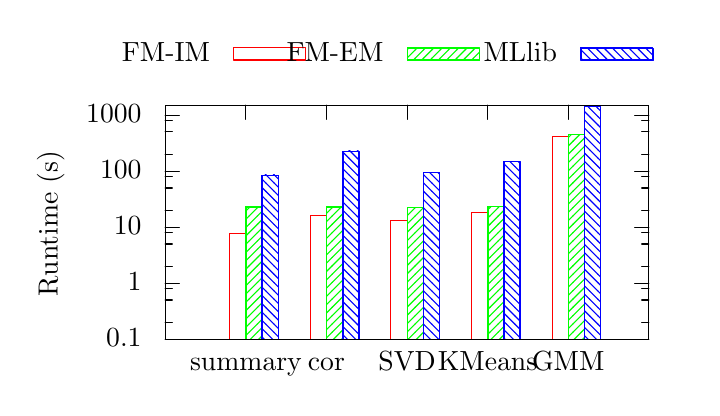
\begin{tikzpicture}[gnuplot]
%% generated with GNUPLOT 4.6p4 (Lua 5.1; terminal rev. 99, script rev. 100)
%% Fri 08 Apr 2016 06:45:40 PM EDT
\path (0.000,0.000) rectangle (8.382,4.572);
\gpcolor{color=gp lt color border}
\gpsetlinetype{gp lt border}
\gpsetlinewidth{1.00}
\draw[gp path] (1.688,0.616)--(1.868,0.616);
\draw[gp path] (7.829,0.616)--(7.649,0.616);
\node[gp node right] at (1.504,0.616) { 0.1};
\draw[gp path] (1.688,0.830)--(1.778,0.830);
\draw[gp path] (7.829,0.830)--(7.739,0.830);
\draw[gp path] (1.688,1.113)--(1.778,1.113);
\draw[gp path] (7.829,1.113)--(7.739,1.113);
\draw[gp path] (1.688,1.258)--(1.778,1.258);
\draw[gp path] (7.829,1.258)--(7.739,1.258);
\draw[gp path] (1.688,1.327)--(1.868,1.327);
\draw[gp path] (7.829,1.327)--(7.649,1.327);
\node[gp node right] at (1.504,1.327) { 1};
\draw[gp path] (1.688,1.542)--(1.778,1.542);
\draw[gp path] (7.829,1.542)--(7.739,1.542);
\draw[gp path] (1.688,1.825)--(1.778,1.825);
\draw[gp path] (7.829,1.825)--(7.739,1.825);
\draw[gp path] (1.688,1.970)--(1.778,1.970);
\draw[gp path] (7.829,1.970)--(7.739,1.970);
\draw[gp path] (1.688,2.039)--(1.868,2.039);
\draw[gp path] (7.829,2.039)--(7.649,2.039);
\node[gp node right] at (1.504,2.039) { 10};
\draw[gp path] (1.688,2.253)--(1.778,2.253);
\draw[gp path] (7.829,2.253)--(7.739,2.253);
\draw[gp path] (1.688,2.536)--(1.778,2.536);
\draw[gp path] (7.829,2.536)--(7.739,2.536);
\draw[gp path] (1.688,2.681)--(1.778,2.681);
\draw[gp path] (7.829,2.681)--(7.739,2.681);
\draw[gp path] (1.688,2.750)--(1.868,2.750);
\draw[gp path] (7.829,2.750)--(7.649,2.750);
\node[gp node right] at (1.504,2.750) { 100};
\draw[gp path] (1.688,2.964)--(1.778,2.964);
\draw[gp path] (7.829,2.964)--(7.739,2.964);
\draw[gp path] (1.688,3.248)--(1.778,3.248);
\draw[gp path] (7.829,3.248)--(7.739,3.248);
\draw[gp path] (1.688,3.393)--(1.778,3.393);
\draw[gp path] (7.829,3.393)--(7.739,3.393);
\draw[gp path] (1.688,3.462)--(1.868,3.462);
\draw[gp path] (7.829,3.462)--(7.649,3.462);
\node[gp node right] at (1.504,3.462) { 1000};
\draw[gp path] (2.712,0.616)--(2.712,0.796);
\draw[gp path] (2.712,3.587)--(2.712,3.407);
\node[gp node center] at (2.712,0.308) {summary};
\draw[gp path] (3.735,0.616)--(3.735,0.796);
\draw[gp path] (3.735,3.587)--(3.735,3.407);
\node[gp node center] at (3.735,0.308) {cor};
\draw[gp path] (4.759,0.616)--(4.759,0.796);
\draw[gp path] (4.759,3.587)--(4.759,3.407);
\node[gp node center] at (4.759,0.308) {SVD};
\draw[gp path] (5.782,0.616)--(5.782,0.796);
\draw[gp path] (5.782,3.587)--(5.782,3.407);
\node[gp node center] at (5.782,0.308) {KMeans};
\draw[gp path] (6.806,0.616)--(6.806,0.796);
\draw[gp path] (6.806,3.587)--(6.806,3.407);
\node[gp node center] at (6.806,0.308) {GMM};
\draw[gp path] (1.688,3.587)--(1.688,0.616)--(7.829,0.616)--(7.829,3.587)--cycle;
\node[gp node center,rotate=-270] at (0.246,2.101) {Runtime (s)};
\node[gp node right] at (2.372,4.238) {FM-IM};
\def\gpfillpath{(2.556,4.161)--(3.472,4.161)--(3.472,4.315)--(2.556,4.315)--cycle}
\gpfill{color=gpbgfillcolor} \gpfillpath;
\gpfill{color=gp lt color 0,gp pattern 0,pattern color=.} \gpfillpath;
\gpcolor{color=gp lt color 0}
\gpsetlinetype{gp lt plot 0}
\draw[gp path] (2.556,4.161)--(3.472,4.161)--(3.472,4.315)--(2.556,4.315)--cycle;
\def\gpfillpath{(2.507,0.616)--(2.713,0.616)--(2.713,1.955)--(2.507,1.955)--cycle}
\gpfill{color=gpbgfillcolor} \gpfillpath;
\gpfill{color=gp lt color 0,gp pattern 0,pattern color=.} \gpfillpath;
\draw[gp path] (2.507,0.616)--(2.507,1.954)--(2.712,1.954)--(2.712,0.616)--cycle;
\def\gpfillpath{(3.530,0.616)--(3.736,0.616)--(3.736,2.185)--(3.530,2.185)--cycle}
\gpfill{color=gpbgfillcolor} \gpfillpath;
\gpfill{color=gp lt color 0,gp pattern 0,pattern color=.} \gpfillpath;
\draw[gp path] (3.530,0.616)--(3.530,2.184)--(3.735,2.184)--(3.735,0.616)--cycle;
\def\gpfillpath{(4.554,0.616)--(4.760,0.616)--(4.760,2.125)--(4.554,2.125)--cycle}
\gpfill{color=gpbgfillcolor} \gpfillpath;
\gpfill{color=gp lt color 0,gp pattern 0,pattern color=.} \gpfillpath;
\draw[gp path] (4.554,0.616)--(4.554,2.124)--(4.759,2.124)--(4.759,0.616)--cycle;
\def\gpfillpath{(5.577,0.616)--(5.783,0.616)--(5.783,2.222)--(5.577,2.222)--cycle}
\gpfill{color=gpbgfillcolor} \gpfillpath;
\gpfill{color=gp lt color 0,gp pattern 0,pattern color=.} \gpfillpath;
\draw[gp path] (5.577,0.616)--(5.577,2.221)--(5.782,2.221)--(5.782,0.616)--cycle;
\def\gpfillpath{(6.601,0.616)--(6.807,0.616)--(6.807,3.191)--(6.601,3.191)--cycle}
\gpfill{color=gpbgfillcolor} \gpfillpath;
\gpfill{color=gp lt color 0,gp pattern 0,pattern color=.} \gpfillpath;
\draw[gp path] (6.601,0.616)--(6.601,3.190)--(6.806,3.190)--(6.806,0.616)--cycle;
\gpcolor{color=gp lt color border}
\node[gp node right] at (4.576,4.238) {FM-EM};
\def\gpfillpath{(4.760,4.161)--(5.676,4.161)--(5.676,4.315)--(4.760,4.315)--cycle}
\gpfill{color=gpbgfillcolor} \gpfillpath;
\gpfill{color=gp lt color 1,gp pattern 1,pattern color=.} \gpfillpath;
\gpcolor{color=gp lt color 1}
\gpsetlinetype{gp lt plot 1}
\draw[gp path] (4.760,4.161)--(5.676,4.161)--(5.676,4.315)--(4.760,4.315)--cycle;
\def\gpfillpath{(2.712,0.616)--(2.917,0.616)--(2.917,2.298)--(2.712,2.298)--cycle}
\gpfill{color=gpbgfillcolor} \gpfillpath;
\gpfill{color=gp lt color 1,gp pattern 1,pattern color=.} \gpfillpath;
\draw[gp path] (2.712,0.616)--(2.712,2.297)--(2.916,2.297)--(2.916,0.616)--cycle;
\def\gpfillpath{(3.735,0.616)--(3.941,0.616)--(3.941,2.298)--(3.735,2.298)--cycle}
\gpfill{color=gpbgfillcolor} \gpfillpath;
\gpfill{color=gp lt color 1,gp pattern 1,pattern color=.} \gpfillpath;
\draw[gp path] (3.735,0.616)--(3.735,2.297)--(3.940,2.297)--(3.940,0.616)--cycle;
\def\gpfillpath{(4.759,0.616)--(4.964,0.616)--(4.964,2.294)--(4.759,2.294)--cycle}
\gpfill{color=gpbgfillcolor} \gpfillpath;
\gpfill{color=gp lt color 1,gp pattern 1,pattern color=.} \gpfillpath;
\draw[gp path] (4.759,0.616)--(4.759,2.293)--(4.963,2.293)--(4.963,0.616)--cycle;
\def\gpfillpath{(5.782,0.616)--(5.988,0.616)--(5.988,2.302)--(5.782,2.302)--cycle}
\gpfill{color=gpbgfillcolor} \gpfillpath;
\gpfill{color=gp lt color 1,gp pattern 1,pattern color=.} \gpfillpath;
\draw[gp path] (5.782,0.616)--(5.782,2.301)--(5.987,2.301)--(5.987,0.616)--cycle;
\def\gpfillpath{(6.806,0.616)--(7.011,0.616)--(7.011,3.216)--(6.806,3.216)--cycle}
\gpfill{color=gpbgfillcolor} \gpfillpath;
\gpfill{color=gp lt color 1,gp pattern 1,pattern color=.} \gpfillpath;
\draw[gp path] (6.806,0.616)--(6.806,3.215)--(7.010,3.215)--(7.010,0.616)--cycle;
\gpcolor{color=gp lt color border}
\node[gp node right] at (6.780,4.238) {MLlib};
\def\gpfillpath{(6.964,4.161)--(7.880,4.161)--(7.880,4.315)--(6.964,4.315)--cycle}
\gpfill{color=gpbgfillcolor} \gpfillpath;
\gpfill{color=gp lt color 2,gp pattern 2,pattern color=.} \gpfillpath;
\gpcolor{color=gp lt color 2}
\gpsetlinetype{gp lt plot 2}
\draw[gp path] (6.964,4.161)--(7.880,4.161)--(7.880,4.315)--(6.964,4.315)--cycle;
\def\gpfillpath{(2.916,0.616)--(3.122,0.616)--(3.122,2.701)--(2.916,2.701)--cycle}
\gpfill{color=gpbgfillcolor} \gpfillpath;
\gpfill{color=gp lt color 2,gp pattern 2,pattern color=.} \gpfillpath;
\draw[gp path] (2.916,0.616)--(2.916,2.700)--(3.121,2.700)--(3.121,0.616)--cycle;
\def\gpfillpath{(3.940,0.616)--(4.145,0.616)--(4.145,3.006)--(3.940,3.006)--cycle}
\gpfill{color=gpbgfillcolor} \gpfillpath;
\gpfill{color=gp lt color 2,gp pattern 2,pattern color=.} \gpfillpath;
\draw[gp path] (3.940,0.616)--(3.940,3.005)--(4.144,3.005)--(4.144,0.616)--cycle;
\def\gpfillpath{(4.963,0.616)--(5.169,0.616)--(5.169,2.739)--(4.963,2.739)--cycle}
\gpfill{color=gpbgfillcolor} \gpfillpath;
\gpfill{color=gp lt color 2,gp pattern 2,pattern color=.} \gpfillpath;
\draw[gp path] (4.963,0.616)--(4.963,2.738)--(5.168,2.738)--(5.168,0.616)--cycle;
\def\gpfillpath{(5.987,0.616)--(6.192,0.616)--(6.192,2.875)--(5.987,2.875)--cycle}
\gpfill{color=gpbgfillcolor} \gpfillpath;
\gpfill{color=gp lt color 2,gp pattern 2,pattern color=.} \gpfillpath;
\draw[gp path] (5.987,0.616)--(5.987,2.874)--(6.191,2.874)--(6.191,0.616)--cycle;
\def\gpfillpath{(7.010,0.616)--(7.216,0.616)--(7.216,3.576)--(7.010,3.576)--cycle}
\gpfill{color=gpbgfillcolor} \gpfillpath;
\gpfill{color=gp lt color 2,gp pattern 2,pattern color=.} \gpfillpath;
\draw[gp path] (7.010,0.616)--(7.010,3.575)--(7.215,3.575)--(7.215,0.616)--cycle;
\gpcolor{color=gp lt color border}
\gpsetlinetype{gp lt border}
\draw[gp path] (1.688,3.587)--(1.688,0.616)--(7.829,0.616)--(7.829,3.587)--cycle;
%% coordinates of the plot area
\gpdefrectangularnode{gp plot 1}{\pgfpoint{1.688cm}{0.616cm}}{\pgfpoint{7.829cm}{3.587cm}}
\end{tikzpicture}
%% gnuplot variables

		\label{perf:rt}
		\vspace{-15pt}
		\caption{Runtime}
	\end{subfigure}

	%\vspace{-5pt}
	\begin{subfigure}{.5\textwidth}
		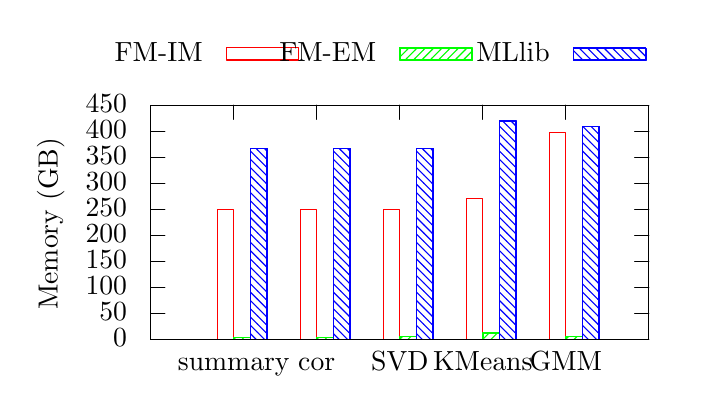
\begin{tikzpicture}[gnuplot]
%% generated with GNUPLOT 4.6p4 (Lua 5.1; terminal rev. 99, script rev. 100)
%% Fri 08 Apr 2016 10:23:19 PM EDT
\path (0.000,0.000) rectangle (8.382,4.572);
\gpcolor{color=gp lt color border}
\gpsetlinetype{gp lt border}
\gpsetlinewidth{1.00}
\draw[gp path] (1.504,0.616)--(1.684,0.616);
\draw[gp path] (7.829,0.616)--(7.649,0.616);
\node[gp node right] at (1.320,0.616) { 0};
\draw[gp path] (1.504,0.946)--(1.684,0.946);
\draw[gp path] (7.829,0.946)--(7.649,0.946);
\node[gp node right] at (1.320,0.946) { 50};
\draw[gp path] (1.504,1.276)--(1.684,1.276);
\draw[gp path] (7.829,1.276)--(7.649,1.276);
\node[gp node right] at (1.320,1.276) { 100};
\draw[gp path] (1.504,1.606)--(1.684,1.606);
\draw[gp path] (7.829,1.606)--(7.649,1.606);
\node[gp node right] at (1.320,1.606) { 150};
\draw[gp path] (1.504,1.936)--(1.684,1.936);
\draw[gp path] (7.829,1.936)--(7.649,1.936);
\node[gp node right] at (1.320,1.936) { 200};
\draw[gp path] (1.504,2.267)--(1.684,2.267);
\draw[gp path] (7.829,2.267)--(7.649,2.267);
\node[gp node right] at (1.320,2.267) { 250};
\draw[gp path] (1.504,2.597)--(1.684,2.597);
\draw[gp path] (7.829,2.597)--(7.649,2.597);
\node[gp node right] at (1.320,2.597) { 300};
\draw[gp path] (1.504,2.927)--(1.684,2.927);
\draw[gp path] (7.829,2.927)--(7.649,2.927);
\node[gp node right] at (1.320,2.927) { 350};
\draw[gp path] (1.504,3.257)--(1.684,3.257);
\draw[gp path] (7.829,3.257)--(7.649,3.257);
\node[gp node right] at (1.320,3.257) { 400};
\draw[gp path] (1.504,3.587)--(1.684,3.587);
\draw[gp path] (7.829,3.587)--(7.649,3.587);
\node[gp node right] at (1.320,3.587) { 450};
\draw[gp path] (2.558,0.616)--(2.558,0.796);
\draw[gp path] (2.558,3.587)--(2.558,3.407);
\node[gp node center] at (2.558,0.308) {summary};
\draw[gp path] (3.612,0.616)--(3.612,0.796);
\draw[gp path] (3.612,3.587)--(3.612,3.407);
\node[gp node center] at (3.612,0.308) {cor};
\draw[gp path] (4.667,0.616)--(4.667,0.796);
\draw[gp path] (4.667,3.587)--(4.667,3.407);
\node[gp node center] at (4.667,0.308) {SVD};
\draw[gp path] (5.721,0.616)--(5.721,0.796);
\draw[gp path] (5.721,3.587)--(5.721,3.407);
\node[gp node center] at (5.721,0.308) {KMeans};
\draw[gp path] (6.775,0.616)--(6.775,0.796);
\draw[gp path] (6.775,3.587)--(6.775,3.407);
\node[gp node center] at (6.775,0.308) {GMM};
\draw[gp path] (1.504,3.587)--(1.504,0.616)--(7.829,0.616)--(7.829,3.587)--cycle;
\node[gp node center,rotate=-270] at (0.246,2.101) {Memory (GB)};
\node[gp node right] at (2.280,4.238) {FM-IM};
\def\gpfillpath{(2.464,4.161)--(3.380,4.161)--(3.380,4.315)--(2.464,4.315)--cycle}
\gpfill{color=gpbgfillcolor} \gpfillpath;
\gpfill{color=gp lt color 0,gp pattern 0,pattern color=.} \gpfillpath;
\gpcolor{color=gp lt color 0}
\gpsetlinetype{gp lt plot 0}
\draw[gp path] (2.464,4.161)--(3.380,4.161)--(3.380,4.315)--(2.464,4.315)--cycle;
\def\gpfillpath{(2.347,0.616)--(2.559,0.616)--(2.559,2.267)--(2.347,2.267)--cycle}
\gpfill{color=gpbgfillcolor} \gpfillpath;
\gpfill{color=gp lt color 0,gp pattern 0,pattern color=.} \gpfillpath;
\draw[gp path] (2.347,0.616)--(2.347,2.266)--(2.558,2.266)--(2.558,0.616)--cycle;
\def\gpfillpath{(3.402,0.616)--(3.613,0.616)--(3.613,2.267)--(3.402,2.267)--cycle}
\gpfill{color=gpbgfillcolor} \gpfillpath;
\gpfill{color=gp lt color 0,gp pattern 0,pattern color=.} \gpfillpath;
\draw[gp path] (3.402,0.616)--(3.402,2.266)--(3.612,2.266)--(3.612,0.616)--cycle;
\def\gpfillpath{(4.456,0.616)--(4.668,0.616)--(4.668,2.267)--(4.456,2.267)--cycle}
\gpfill{color=gpbgfillcolor} \gpfillpath;
\gpfill{color=gp lt color 0,gp pattern 0,pattern color=.} \gpfillpath;
\draw[gp path] (4.456,0.616)--(4.456,2.266)--(4.667,2.266)--(4.667,0.616)--cycle;
\def\gpfillpath{(5.510,0.616)--(5.722,0.616)--(5.722,2.402)--(5.510,2.402)--cycle}
\gpfill{color=gpbgfillcolor} \gpfillpath;
\gpfill{color=gp lt color 0,gp pattern 0,pattern color=.} \gpfillpath;
\draw[gp path] (5.510,0.616)--(5.510,2.401)--(5.721,2.401)--(5.721,0.616)--cycle;
\def\gpfillpath{(6.564,0.616)--(6.776,0.616)--(6.776,3.238)--(6.564,3.238)--cycle}
\gpfill{color=gpbgfillcolor} \gpfillpath;
\gpfill{color=gp lt color 0,gp pattern 0,pattern color=.} \gpfillpath;
\draw[gp path] (6.564,0.616)--(6.564,3.237)--(6.775,3.237)--(6.775,0.616)--cycle;
\gpcolor{color=gp lt color border}
\node[gp node right] at (4.484,4.238) {FM-EM};
\def\gpfillpath{(4.668,4.161)--(5.584,4.161)--(5.584,4.315)--(4.668,4.315)--cycle}
\gpfill{color=gpbgfillcolor} \gpfillpath;
\gpfill{color=gp lt color 1,gp pattern 1,pattern color=.} \gpfillpath;
\gpcolor{color=gp lt color 1}
\gpsetlinetype{gp lt plot 1}
\draw[gp path] (4.668,4.161)--(5.584,4.161)--(5.584,4.315)--(4.668,4.315)--cycle;
\def\gpfillpath{(2.558,0.616)--(2.770,0.616)--(2.770,0.642)--(2.558,0.642)--cycle}
\gpfill{color=gpbgfillcolor} \gpfillpath;
\gpfill{color=gp lt color 1,gp pattern 1,pattern color=.} \gpfillpath;
\draw[gp path] (2.558,0.616)--(2.558,0.641)--(2.769,0.641)--(2.769,0.616)--cycle;
\def\gpfillpath{(3.612,0.616)--(3.824,0.616)--(3.824,0.643)--(3.612,0.643)--cycle}
\gpfill{color=gpbgfillcolor} \gpfillpath;
\gpfill{color=gp lt color 1,gp pattern 1,pattern color=.} \gpfillpath;
\draw[gp path] (3.612,0.616)--(3.612,0.642)--(3.823,0.642)--(3.823,0.616)--cycle;
\def\gpfillpath{(4.667,0.616)--(4.878,0.616)--(4.878,0.651)--(4.667,0.651)--cycle}
\gpfill{color=gpbgfillcolor} \gpfillpath;
\gpfill{color=gp lt color 1,gp pattern 1,pattern color=.} \gpfillpath;
\draw[gp path] (4.667,0.616)--(4.667,0.650)--(4.877,0.650)--(4.877,0.616)--cycle;
\def\gpfillpath{(5.721,0.616)--(5.933,0.616)--(5.933,0.696)--(5.721,0.696)--cycle}
\gpfill{color=gpbgfillcolor} \gpfillpath;
\gpfill{color=gp lt color 1,gp pattern 1,pattern color=.} \gpfillpath;
\draw[gp path] (5.721,0.616)--(5.721,0.695)--(5.932,0.695)--(5.932,0.616)--cycle;
\def\gpfillpath{(6.775,0.616)--(6.987,0.616)--(6.987,0.656)--(6.775,0.656)--cycle}
\gpfill{color=gpbgfillcolor} \gpfillpath;
\gpfill{color=gp lt color 1,gp pattern 1,pattern color=.} \gpfillpath;
\draw[gp path] (6.775,0.616)--(6.775,0.655)--(6.986,0.655)--(6.986,0.616)--cycle;
\gpcolor{color=gp lt color border}
\node[gp node right] at (6.688,4.238) {MLlib};
\def\gpfillpath{(6.872,4.161)--(7.788,4.161)--(7.788,4.315)--(6.872,4.315)--cycle}
\gpfill{color=gpbgfillcolor} \gpfillpath;
\gpfill{color=gp lt color 2,gp pattern 2,pattern color=.} \gpfillpath;
\gpcolor{color=gp lt color 2}
\gpsetlinetype{gp lt plot 2}
\draw[gp path] (6.872,4.161)--(7.788,4.161)--(7.788,4.315)--(6.872,4.315)--cycle;
\def\gpfillpath{(2.769,0.616)--(2.981,0.616)--(2.981,3.037)--(2.769,3.037)--cycle}
\gpfill{color=gpbgfillcolor} \gpfillpath;
\gpfill{color=gp lt color 2,gp pattern 2,pattern color=.} \gpfillpath;
\draw[gp path] (2.769,0.616)--(2.769,3.036)--(2.980,3.036)--(2.980,0.616)--cycle;
\def\gpfillpath{(3.823,0.616)--(4.035,0.616)--(4.035,3.037)--(3.823,3.037)--cycle}
\gpfill{color=gpbgfillcolor} \gpfillpath;
\gpfill{color=gp lt color 2,gp pattern 2,pattern color=.} \gpfillpath;
\draw[gp path] (3.823,0.616)--(3.823,3.036)--(4.034,3.036)--(4.034,0.616)--cycle;
\def\gpfillpath{(4.877,0.616)--(5.089,0.616)--(5.089,3.037)--(4.877,3.037)--cycle}
\gpfill{color=gpbgfillcolor} \gpfillpath;
\gpfill{color=gp lt color 2,gp pattern 2,pattern color=.} \gpfillpath;
\draw[gp path] (4.877,0.616)--(4.877,3.036)--(5.088,3.036)--(5.088,0.616)--cycle;
\def\gpfillpath{(5.932,0.616)--(6.143,0.616)--(6.143,3.390)--(5.932,3.390)--cycle}
\gpfill{color=gpbgfillcolor} \gpfillpath;
\gpfill{color=gp lt color 2,gp pattern 2,pattern color=.} \gpfillpath;
\draw[gp path] (5.932,0.616)--(5.932,3.389)--(6.142,3.389)--(6.142,0.616)--cycle;
\def\gpfillpath{(6.986,0.616)--(7.198,0.616)--(7.198,3.321)--(6.986,3.321)--cycle}
\gpfill{color=gpbgfillcolor} \gpfillpath;
\gpfill{color=gp lt color 2,gp pattern 2,pattern color=.} \gpfillpath;
\draw[gp path] (6.986,0.616)--(6.986,3.320)--(7.197,3.320)--(7.197,0.616)--cycle;
\gpcolor{color=gp lt color border}
\gpsetlinetype{gp lt border}
\draw[gp path] (1.504,3.587)--(1.504,0.616)--(7.829,0.616)--(7.829,3.587)--cycle;
%% coordinates of the plot area
\gpdefrectangularnode{gp plot 1}{\pgfpoint{1.504cm}{0.616cm}}{\pgfpoint{7.829cm}{3.587cm}}
\end{tikzpicture}
%% gnuplot variables

		\label{perf:mem}
		\vspace{-15pt}
		\caption{Memory consumption}
	\end{subfigure}
	\caption{The performance and memory consumption of FlashMatrix both
		in memory (FM-IM) and on SSDs (FM-EM) compared with Spark MLlib
		on the MixGaussian-1B matrix.}
	\label{perf:fm}
\end{figure}

%\begin{figure}
%	\begin{center}
%		\footnotesize
%		\vspace{-15pt}
%		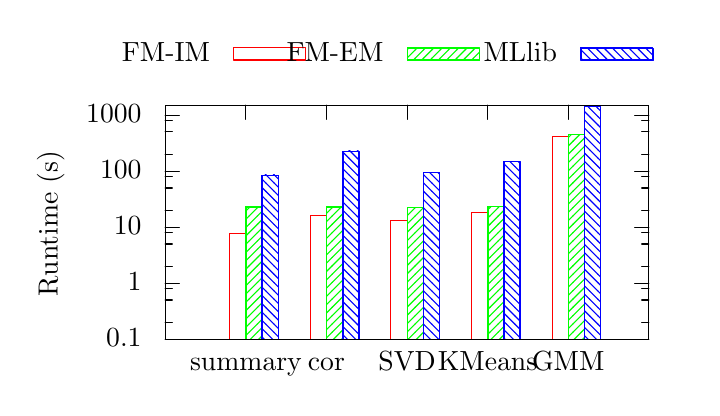
\begin{tikzpicture}[gnuplot]
%% generated with GNUPLOT 4.6p4 (Lua 5.1; terminal rev. 99, script rev. 100)
%% Fri 08 Apr 2016 06:45:40 PM EDT
\path (0.000,0.000) rectangle (8.382,4.572);
\gpcolor{color=gp lt color border}
\gpsetlinetype{gp lt border}
\gpsetlinewidth{1.00}
\draw[gp path] (1.688,0.616)--(1.868,0.616);
\draw[gp path] (7.829,0.616)--(7.649,0.616);
\node[gp node right] at (1.504,0.616) { 0.1};
\draw[gp path] (1.688,0.830)--(1.778,0.830);
\draw[gp path] (7.829,0.830)--(7.739,0.830);
\draw[gp path] (1.688,1.113)--(1.778,1.113);
\draw[gp path] (7.829,1.113)--(7.739,1.113);
\draw[gp path] (1.688,1.258)--(1.778,1.258);
\draw[gp path] (7.829,1.258)--(7.739,1.258);
\draw[gp path] (1.688,1.327)--(1.868,1.327);
\draw[gp path] (7.829,1.327)--(7.649,1.327);
\node[gp node right] at (1.504,1.327) { 1};
\draw[gp path] (1.688,1.542)--(1.778,1.542);
\draw[gp path] (7.829,1.542)--(7.739,1.542);
\draw[gp path] (1.688,1.825)--(1.778,1.825);
\draw[gp path] (7.829,1.825)--(7.739,1.825);
\draw[gp path] (1.688,1.970)--(1.778,1.970);
\draw[gp path] (7.829,1.970)--(7.739,1.970);
\draw[gp path] (1.688,2.039)--(1.868,2.039);
\draw[gp path] (7.829,2.039)--(7.649,2.039);
\node[gp node right] at (1.504,2.039) { 10};
\draw[gp path] (1.688,2.253)--(1.778,2.253);
\draw[gp path] (7.829,2.253)--(7.739,2.253);
\draw[gp path] (1.688,2.536)--(1.778,2.536);
\draw[gp path] (7.829,2.536)--(7.739,2.536);
\draw[gp path] (1.688,2.681)--(1.778,2.681);
\draw[gp path] (7.829,2.681)--(7.739,2.681);
\draw[gp path] (1.688,2.750)--(1.868,2.750);
\draw[gp path] (7.829,2.750)--(7.649,2.750);
\node[gp node right] at (1.504,2.750) { 100};
\draw[gp path] (1.688,2.964)--(1.778,2.964);
\draw[gp path] (7.829,2.964)--(7.739,2.964);
\draw[gp path] (1.688,3.248)--(1.778,3.248);
\draw[gp path] (7.829,3.248)--(7.739,3.248);
\draw[gp path] (1.688,3.393)--(1.778,3.393);
\draw[gp path] (7.829,3.393)--(7.739,3.393);
\draw[gp path] (1.688,3.462)--(1.868,3.462);
\draw[gp path] (7.829,3.462)--(7.649,3.462);
\node[gp node right] at (1.504,3.462) { 1000};
\draw[gp path] (2.712,0.616)--(2.712,0.796);
\draw[gp path] (2.712,3.587)--(2.712,3.407);
\node[gp node center] at (2.712,0.308) {summary};
\draw[gp path] (3.735,0.616)--(3.735,0.796);
\draw[gp path] (3.735,3.587)--(3.735,3.407);
\node[gp node center] at (3.735,0.308) {cor};
\draw[gp path] (4.759,0.616)--(4.759,0.796);
\draw[gp path] (4.759,3.587)--(4.759,3.407);
\node[gp node center] at (4.759,0.308) {SVD};
\draw[gp path] (5.782,0.616)--(5.782,0.796);
\draw[gp path] (5.782,3.587)--(5.782,3.407);
\node[gp node center] at (5.782,0.308) {KMeans};
\draw[gp path] (6.806,0.616)--(6.806,0.796);
\draw[gp path] (6.806,3.587)--(6.806,3.407);
\node[gp node center] at (6.806,0.308) {GMM};
\draw[gp path] (1.688,3.587)--(1.688,0.616)--(7.829,0.616)--(7.829,3.587)--cycle;
\node[gp node center,rotate=-270] at (0.246,2.101) {Runtime (s)};
\node[gp node right] at (2.372,4.238) {FM-IM};
\def\gpfillpath{(2.556,4.161)--(3.472,4.161)--(3.472,4.315)--(2.556,4.315)--cycle}
\gpfill{color=gpbgfillcolor} \gpfillpath;
\gpfill{color=gp lt color 0,gp pattern 0,pattern color=.} \gpfillpath;
\gpcolor{color=gp lt color 0}
\gpsetlinetype{gp lt plot 0}
\draw[gp path] (2.556,4.161)--(3.472,4.161)--(3.472,4.315)--(2.556,4.315)--cycle;
\def\gpfillpath{(2.507,0.616)--(2.713,0.616)--(2.713,1.955)--(2.507,1.955)--cycle}
\gpfill{color=gpbgfillcolor} \gpfillpath;
\gpfill{color=gp lt color 0,gp pattern 0,pattern color=.} \gpfillpath;
\draw[gp path] (2.507,0.616)--(2.507,1.954)--(2.712,1.954)--(2.712,0.616)--cycle;
\def\gpfillpath{(3.530,0.616)--(3.736,0.616)--(3.736,2.185)--(3.530,2.185)--cycle}
\gpfill{color=gpbgfillcolor} \gpfillpath;
\gpfill{color=gp lt color 0,gp pattern 0,pattern color=.} \gpfillpath;
\draw[gp path] (3.530,0.616)--(3.530,2.184)--(3.735,2.184)--(3.735,0.616)--cycle;
\def\gpfillpath{(4.554,0.616)--(4.760,0.616)--(4.760,2.125)--(4.554,2.125)--cycle}
\gpfill{color=gpbgfillcolor} \gpfillpath;
\gpfill{color=gp lt color 0,gp pattern 0,pattern color=.} \gpfillpath;
\draw[gp path] (4.554,0.616)--(4.554,2.124)--(4.759,2.124)--(4.759,0.616)--cycle;
\def\gpfillpath{(5.577,0.616)--(5.783,0.616)--(5.783,2.222)--(5.577,2.222)--cycle}
\gpfill{color=gpbgfillcolor} \gpfillpath;
\gpfill{color=gp lt color 0,gp pattern 0,pattern color=.} \gpfillpath;
\draw[gp path] (5.577,0.616)--(5.577,2.221)--(5.782,2.221)--(5.782,0.616)--cycle;
\def\gpfillpath{(6.601,0.616)--(6.807,0.616)--(6.807,3.191)--(6.601,3.191)--cycle}
\gpfill{color=gpbgfillcolor} \gpfillpath;
\gpfill{color=gp lt color 0,gp pattern 0,pattern color=.} \gpfillpath;
\draw[gp path] (6.601,0.616)--(6.601,3.190)--(6.806,3.190)--(6.806,0.616)--cycle;
\gpcolor{color=gp lt color border}
\node[gp node right] at (4.576,4.238) {FM-EM};
\def\gpfillpath{(4.760,4.161)--(5.676,4.161)--(5.676,4.315)--(4.760,4.315)--cycle}
\gpfill{color=gpbgfillcolor} \gpfillpath;
\gpfill{color=gp lt color 1,gp pattern 1,pattern color=.} \gpfillpath;
\gpcolor{color=gp lt color 1}
\gpsetlinetype{gp lt plot 1}
\draw[gp path] (4.760,4.161)--(5.676,4.161)--(5.676,4.315)--(4.760,4.315)--cycle;
\def\gpfillpath{(2.712,0.616)--(2.917,0.616)--(2.917,2.298)--(2.712,2.298)--cycle}
\gpfill{color=gpbgfillcolor} \gpfillpath;
\gpfill{color=gp lt color 1,gp pattern 1,pattern color=.} \gpfillpath;
\draw[gp path] (2.712,0.616)--(2.712,2.297)--(2.916,2.297)--(2.916,0.616)--cycle;
\def\gpfillpath{(3.735,0.616)--(3.941,0.616)--(3.941,2.298)--(3.735,2.298)--cycle}
\gpfill{color=gpbgfillcolor} \gpfillpath;
\gpfill{color=gp lt color 1,gp pattern 1,pattern color=.} \gpfillpath;
\draw[gp path] (3.735,0.616)--(3.735,2.297)--(3.940,2.297)--(3.940,0.616)--cycle;
\def\gpfillpath{(4.759,0.616)--(4.964,0.616)--(4.964,2.294)--(4.759,2.294)--cycle}
\gpfill{color=gpbgfillcolor} \gpfillpath;
\gpfill{color=gp lt color 1,gp pattern 1,pattern color=.} \gpfillpath;
\draw[gp path] (4.759,0.616)--(4.759,2.293)--(4.963,2.293)--(4.963,0.616)--cycle;
\def\gpfillpath{(5.782,0.616)--(5.988,0.616)--(5.988,2.302)--(5.782,2.302)--cycle}
\gpfill{color=gpbgfillcolor} \gpfillpath;
\gpfill{color=gp lt color 1,gp pattern 1,pattern color=.} \gpfillpath;
\draw[gp path] (5.782,0.616)--(5.782,2.301)--(5.987,2.301)--(5.987,0.616)--cycle;
\def\gpfillpath{(6.806,0.616)--(7.011,0.616)--(7.011,3.216)--(6.806,3.216)--cycle}
\gpfill{color=gpbgfillcolor} \gpfillpath;
\gpfill{color=gp lt color 1,gp pattern 1,pattern color=.} \gpfillpath;
\draw[gp path] (6.806,0.616)--(6.806,3.215)--(7.010,3.215)--(7.010,0.616)--cycle;
\gpcolor{color=gp lt color border}
\node[gp node right] at (6.780,4.238) {MLlib};
\def\gpfillpath{(6.964,4.161)--(7.880,4.161)--(7.880,4.315)--(6.964,4.315)--cycle}
\gpfill{color=gpbgfillcolor} \gpfillpath;
\gpfill{color=gp lt color 2,gp pattern 2,pattern color=.} \gpfillpath;
\gpcolor{color=gp lt color 2}
\gpsetlinetype{gp lt plot 2}
\draw[gp path] (6.964,4.161)--(7.880,4.161)--(7.880,4.315)--(6.964,4.315)--cycle;
\def\gpfillpath{(2.916,0.616)--(3.122,0.616)--(3.122,2.701)--(2.916,2.701)--cycle}
\gpfill{color=gpbgfillcolor} \gpfillpath;
\gpfill{color=gp lt color 2,gp pattern 2,pattern color=.} \gpfillpath;
\draw[gp path] (2.916,0.616)--(2.916,2.700)--(3.121,2.700)--(3.121,0.616)--cycle;
\def\gpfillpath{(3.940,0.616)--(4.145,0.616)--(4.145,3.006)--(3.940,3.006)--cycle}
\gpfill{color=gpbgfillcolor} \gpfillpath;
\gpfill{color=gp lt color 2,gp pattern 2,pattern color=.} \gpfillpath;
\draw[gp path] (3.940,0.616)--(3.940,3.005)--(4.144,3.005)--(4.144,0.616)--cycle;
\def\gpfillpath{(4.963,0.616)--(5.169,0.616)--(5.169,2.739)--(4.963,2.739)--cycle}
\gpfill{color=gpbgfillcolor} \gpfillpath;
\gpfill{color=gp lt color 2,gp pattern 2,pattern color=.} \gpfillpath;
\draw[gp path] (4.963,0.616)--(4.963,2.738)--(5.168,2.738)--(5.168,0.616)--cycle;
\def\gpfillpath{(5.987,0.616)--(6.192,0.616)--(6.192,2.875)--(5.987,2.875)--cycle}
\gpfill{color=gpbgfillcolor} \gpfillpath;
\gpfill{color=gp lt color 2,gp pattern 2,pattern color=.} \gpfillpath;
\draw[gp path] (5.987,0.616)--(5.987,2.874)--(6.191,2.874)--(6.191,0.616)--cycle;
\def\gpfillpath{(7.010,0.616)--(7.216,0.616)--(7.216,3.576)--(7.010,3.576)--cycle}
\gpfill{color=gpbgfillcolor} \gpfillpath;
\gpfill{color=gp lt color 2,gp pattern 2,pattern color=.} \gpfillpath;
\draw[gp path] (7.010,0.616)--(7.010,3.575)--(7.215,3.575)--(7.215,0.616)--cycle;
\gpcolor{color=gp lt color border}
\gpsetlinetype{gp lt border}
\draw[gp path] (1.688,3.587)--(1.688,0.616)--(7.829,0.616)--(7.829,3.587)--cycle;
%% coordinates of the plot area
\gpdefrectangularnode{gp plot 1}{\pgfpoint{1.688cm}{0.616cm}}{\pgfpoint{7.829cm}{3.587cm}}
\end{tikzpicture}
%% gnuplot variables

%		\vspace{-15pt}
%		\caption{The performance of FlashMatrix both in memory and on SSDs
%			compared with Spark MLlib on a matrix with one billion rows and
%		32 columns.}
%		\label{perf:fm}
%	\end{center}
%\end{figure}

FlashMatrix both in memory and on SSDs outperforms Spark MLlib significantly
in all applications (Figure \ref{perf:fm} (a)). For some applications
such as correlation, SVD and GMM, even though both FlashMatrix and MLlib
implementations heavily rely on BLAS for matrix multiplication, FlashMatrix
outperforms MLlib significantly owing to our heavy optimizations on GenOps
such as aggressive matrix operation fusion and VUDFs. In contrast, MLlib
materializes operations such as aggregation separately and implements
non-BLAS operations with Scala.
%SVD is the only application whose FlashMatrix
%implementation does not outperform the one in MLlib when being executed out of
%core because this application requires to read the entire matrix multiple times
%and output a large matrix.

%\begin{figure}
%	\begin{center}
%		\footnotesize
%		\vspace{-15pt}
%		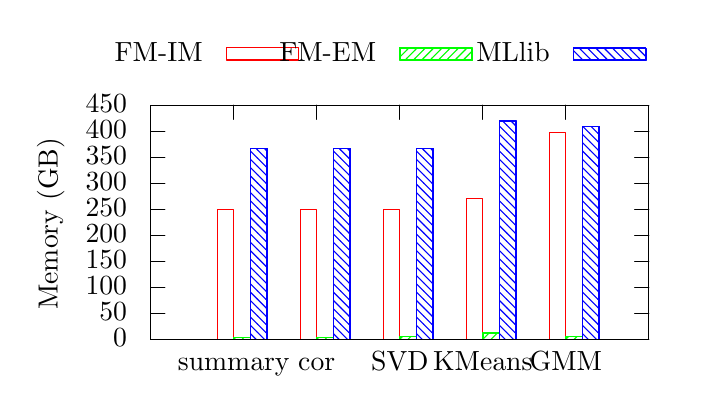
\begin{tikzpicture}[gnuplot]
%% generated with GNUPLOT 4.6p4 (Lua 5.1; terminal rev. 99, script rev. 100)
%% Fri 08 Apr 2016 10:23:19 PM EDT
\path (0.000,0.000) rectangle (8.382,4.572);
\gpcolor{color=gp lt color border}
\gpsetlinetype{gp lt border}
\gpsetlinewidth{1.00}
\draw[gp path] (1.504,0.616)--(1.684,0.616);
\draw[gp path] (7.829,0.616)--(7.649,0.616);
\node[gp node right] at (1.320,0.616) { 0};
\draw[gp path] (1.504,0.946)--(1.684,0.946);
\draw[gp path] (7.829,0.946)--(7.649,0.946);
\node[gp node right] at (1.320,0.946) { 50};
\draw[gp path] (1.504,1.276)--(1.684,1.276);
\draw[gp path] (7.829,1.276)--(7.649,1.276);
\node[gp node right] at (1.320,1.276) { 100};
\draw[gp path] (1.504,1.606)--(1.684,1.606);
\draw[gp path] (7.829,1.606)--(7.649,1.606);
\node[gp node right] at (1.320,1.606) { 150};
\draw[gp path] (1.504,1.936)--(1.684,1.936);
\draw[gp path] (7.829,1.936)--(7.649,1.936);
\node[gp node right] at (1.320,1.936) { 200};
\draw[gp path] (1.504,2.267)--(1.684,2.267);
\draw[gp path] (7.829,2.267)--(7.649,2.267);
\node[gp node right] at (1.320,2.267) { 250};
\draw[gp path] (1.504,2.597)--(1.684,2.597);
\draw[gp path] (7.829,2.597)--(7.649,2.597);
\node[gp node right] at (1.320,2.597) { 300};
\draw[gp path] (1.504,2.927)--(1.684,2.927);
\draw[gp path] (7.829,2.927)--(7.649,2.927);
\node[gp node right] at (1.320,2.927) { 350};
\draw[gp path] (1.504,3.257)--(1.684,3.257);
\draw[gp path] (7.829,3.257)--(7.649,3.257);
\node[gp node right] at (1.320,3.257) { 400};
\draw[gp path] (1.504,3.587)--(1.684,3.587);
\draw[gp path] (7.829,3.587)--(7.649,3.587);
\node[gp node right] at (1.320,3.587) { 450};
\draw[gp path] (2.558,0.616)--(2.558,0.796);
\draw[gp path] (2.558,3.587)--(2.558,3.407);
\node[gp node center] at (2.558,0.308) {summary};
\draw[gp path] (3.612,0.616)--(3.612,0.796);
\draw[gp path] (3.612,3.587)--(3.612,3.407);
\node[gp node center] at (3.612,0.308) {cor};
\draw[gp path] (4.667,0.616)--(4.667,0.796);
\draw[gp path] (4.667,3.587)--(4.667,3.407);
\node[gp node center] at (4.667,0.308) {SVD};
\draw[gp path] (5.721,0.616)--(5.721,0.796);
\draw[gp path] (5.721,3.587)--(5.721,3.407);
\node[gp node center] at (5.721,0.308) {KMeans};
\draw[gp path] (6.775,0.616)--(6.775,0.796);
\draw[gp path] (6.775,3.587)--(6.775,3.407);
\node[gp node center] at (6.775,0.308) {GMM};
\draw[gp path] (1.504,3.587)--(1.504,0.616)--(7.829,0.616)--(7.829,3.587)--cycle;
\node[gp node center,rotate=-270] at (0.246,2.101) {Memory (GB)};
\node[gp node right] at (2.280,4.238) {FM-IM};
\def\gpfillpath{(2.464,4.161)--(3.380,4.161)--(3.380,4.315)--(2.464,4.315)--cycle}
\gpfill{color=gpbgfillcolor} \gpfillpath;
\gpfill{color=gp lt color 0,gp pattern 0,pattern color=.} \gpfillpath;
\gpcolor{color=gp lt color 0}
\gpsetlinetype{gp lt plot 0}
\draw[gp path] (2.464,4.161)--(3.380,4.161)--(3.380,4.315)--(2.464,4.315)--cycle;
\def\gpfillpath{(2.347,0.616)--(2.559,0.616)--(2.559,2.267)--(2.347,2.267)--cycle}
\gpfill{color=gpbgfillcolor} \gpfillpath;
\gpfill{color=gp lt color 0,gp pattern 0,pattern color=.} \gpfillpath;
\draw[gp path] (2.347,0.616)--(2.347,2.266)--(2.558,2.266)--(2.558,0.616)--cycle;
\def\gpfillpath{(3.402,0.616)--(3.613,0.616)--(3.613,2.267)--(3.402,2.267)--cycle}
\gpfill{color=gpbgfillcolor} \gpfillpath;
\gpfill{color=gp lt color 0,gp pattern 0,pattern color=.} \gpfillpath;
\draw[gp path] (3.402,0.616)--(3.402,2.266)--(3.612,2.266)--(3.612,0.616)--cycle;
\def\gpfillpath{(4.456,0.616)--(4.668,0.616)--(4.668,2.267)--(4.456,2.267)--cycle}
\gpfill{color=gpbgfillcolor} \gpfillpath;
\gpfill{color=gp lt color 0,gp pattern 0,pattern color=.} \gpfillpath;
\draw[gp path] (4.456,0.616)--(4.456,2.266)--(4.667,2.266)--(4.667,0.616)--cycle;
\def\gpfillpath{(5.510,0.616)--(5.722,0.616)--(5.722,2.402)--(5.510,2.402)--cycle}
\gpfill{color=gpbgfillcolor} \gpfillpath;
\gpfill{color=gp lt color 0,gp pattern 0,pattern color=.} \gpfillpath;
\draw[gp path] (5.510,0.616)--(5.510,2.401)--(5.721,2.401)--(5.721,0.616)--cycle;
\def\gpfillpath{(6.564,0.616)--(6.776,0.616)--(6.776,3.238)--(6.564,3.238)--cycle}
\gpfill{color=gpbgfillcolor} \gpfillpath;
\gpfill{color=gp lt color 0,gp pattern 0,pattern color=.} \gpfillpath;
\draw[gp path] (6.564,0.616)--(6.564,3.237)--(6.775,3.237)--(6.775,0.616)--cycle;
\gpcolor{color=gp lt color border}
\node[gp node right] at (4.484,4.238) {FM-EM};
\def\gpfillpath{(4.668,4.161)--(5.584,4.161)--(5.584,4.315)--(4.668,4.315)--cycle}
\gpfill{color=gpbgfillcolor} \gpfillpath;
\gpfill{color=gp lt color 1,gp pattern 1,pattern color=.} \gpfillpath;
\gpcolor{color=gp lt color 1}
\gpsetlinetype{gp lt plot 1}
\draw[gp path] (4.668,4.161)--(5.584,4.161)--(5.584,4.315)--(4.668,4.315)--cycle;
\def\gpfillpath{(2.558,0.616)--(2.770,0.616)--(2.770,0.642)--(2.558,0.642)--cycle}
\gpfill{color=gpbgfillcolor} \gpfillpath;
\gpfill{color=gp lt color 1,gp pattern 1,pattern color=.} \gpfillpath;
\draw[gp path] (2.558,0.616)--(2.558,0.641)--(2.769,0.641)--(2.769,0.616)--cycle;
\def\gpfillpath{(3.612,0.616)--(3.824,0.616)--(3.824,0.643)--(3.612,0.643)--cycle}
\gpfill{color=gpbgfillcolor} \gpfillpath;
\gpfill{color=gp lt color 1,gp pattern 1,pattern color=.} \gpfillpath;
\draw[gp path] (3.612,0.616)--(3.612,0.642)--(3.823,0.642)--(3.823,0.616)--cycle;
\def\gpfillpath{(4.667,0.616)--(4.878,0.616)--(4.878,0.651)--(4.667,0.651)--cycle}
\gpfill{color=gpbgfillcolor} \gpfillpath;
\gpfill{color=gp lt color 1,gp pattern 1,pattern color=.} \gpfillpath;
\draw[gp path] (4.667,0.616)--(4.667,0.650)--(4.877,0.650)--(4.877,0.616)--cycle;
\def\gpfillpath{(5.721,0.616)--(5.933,0.616)--(5.933,0.696)--(5.721,0.696)--cycle}
\gpfill{color=gpbgfillcolor} \gpfillpath;
\gpfill{color=gp lt color 1,gp pattern 1,pattern color=.} \gpfillpath;
\draw[gp path] (5.721,0.616)--(5.721,0.695)--(5.932,0.695)--(5.932,0.616)--cycle;
\def\gpfillpath{(6.775,0.616)--(6.987,0.616)--(6.987,0.656)--(6.775,0.656)--cycle}
\gpfill{color=gpbgfillcolor} \gpfillpath;
\gpfill{color=gp lt color 1,gp pattern 1,pattern color=.} \gpfillpath;
\draw[gp path] (6.775,0.616)--(6.775,0.655)--(6.986,0.655)--(6.986,0.616)--cycle;
\gpcolor{color=gp lt color border}
\node[gp node right] at (6.688,4.238) {MLlib};
\def\gpfillpath{(6.872,4.161)--(7.788,4.161)--(7.788,4.315)--(6.872,4.315)--cycle}
\gpfill{color=gpbgfillcolor} \gpfillpath;
\gpfill{color=gp lt color 2,gp pattern 2,pattern color=.} \gpfillpath;
\gpcolor{color=gp lt color 2}
\gpsetlinetype{gp lt plot 2}
\draw[gp path] (6.872,4.161)--(7.788,4.161)--(7.788,4.315)--(6.872,4.315)--cycle;
\def\gpfillpath{(2.769,0.616)--(2.981,0.616)--(2.981,3.037)--(2.769,3.037)--cycle}
\gpfill{color=gpbgfillcolor} \gpfillpath;
\gpfill{color=gp lt color 2,gp pattern 2,pattern color=.} \gpfillpath;
\draw[gp path] (2.769,0.616)--(2.769,3.036)--(2.980,3.036)--(2.980,0.616)--cycle;
\def\gpfillpath{(3.823,0.616)--(4.035,0.616)--(4.035,3.037)--(3.823,3.037)--cycle}
\gpfill{color=gpbgfillcolor} \gpfillpath;
\gpfill{color=gp lt color 2,gp pattern 2,pattern color=.} \gpfillpath;
\draw[gp path] (3.823,0.616)--(3.823,3.036)--(4.034,3.036)--(4.034,0.616)--cycle;
\def\gpfillpath{(4.877,0.616)--(5.089,0.616)--(5.089,3.037)--(4.877,3.037)--cycle}
\gpfill{color=gpbgfillcolor} \gpfillpath;
\gpfill{color=gp lt color 2,gp pattern 2,pattern color=.} \gpfillpath;
\draw[gp path] (4.877,0.616)--(4.877,3.036)--(5.088,3.036)--(5.088,0.616)--cycle;
\def\gpfillpath{(5.932,0.616)--(6.143,0.616)--(6.143,3.390)--(5.932,3.390)--cycle}
\gpfill{color=gpbgfillcolor} \gpfillpath;
\gpfill{color=gp lt color 2,gp pattern 2,pattern color=.} \gpfillpath;
\draw[gp path] (5.932,0.616)--(5.932,3.389)--(6.142,3.389)--(6.142,0.616)--cycle;
\def\gpfillpath{(6.986,0.616)--(7.198,0.616)--(7.198,3.321)--(6.986,3.321)--cycle}
\gpfill{color=gpbgfillcolor} \gpfillpath;
\gpfill{color=gp lt color 2,gp pattern 2,pattern color=.} \gpfillpath;
\draw[gp path] (6.986,0.616)--(6.986,3.320)--(7.197,3.320)--(7.197,0.616)--cycle;
\gpcolor{color=gp lt color border}
\gpsetlinetype{gp lt border}
\draw[gp path] (1.504,3.587)--(1.504,0.616)--(7.829,0.616)--(7.829,3.587)--cycle;
%% coordinates of the plot area
\gpdefrectangularnode{gp plot 1}{\pgfpoint{1.504cm}{0.616cm}}{\pgfpoint{7.829cm}{3.587cm}}
\end{tikzpicture}
%% gnuplot variables

%		\vspace{-15pt}
%		\caption{The memory consumption of FlashMatrix in memory and on SSDs
%		as well as Spark MLlib on a matrix with one billion rows and 32 columns.}
%		\label{perf:mem}
%	\end{center}
%\end{figure}

Even though FlashMatrix provides a matrix-oriented functional programming
interface, it easily scales to datasets with billions of data points and its
scalability is bound by the capacity of SSDs (Figure \ref{perf:fm} (b)).
For out-of-core execution, FlashMatrix keeps large matrices on
SSDs and has a very small memory footprint. The functional programming
interface generates a new matrix in each matrix operation, which potentially
leads to high memory consumption. Owing to lazy evaluation,
FlashMatrix does not store majority of matrices in the computation physically.
As such, its in-memory execution barely increases memory consumption from
the minimum memory requirement of the applications. This indicates that
the out-of-core execution consumes small space on SSDs, which leads to
very high scalability.

\begin{figure}
	\begin{center}
		\footnotesize
		\vspace{-15pt}
		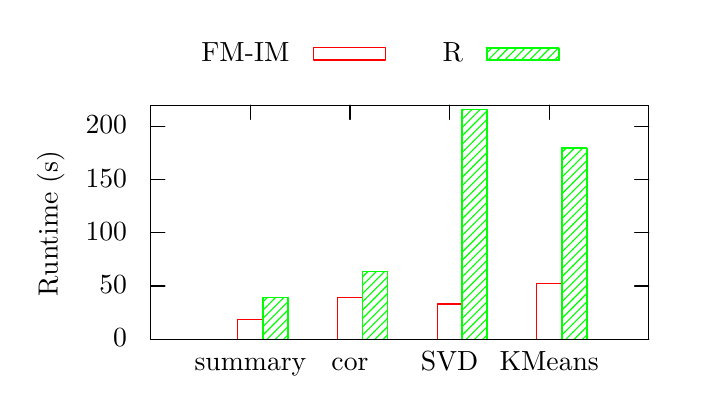
\begin{tikzpicture}[gnuplot]
%% generated with GNUPLOT 4.6p4 (Lua 5.1; terminal rev. 99, script rev. 100)
%% Sat 02 Apr 2016 10:17:07 PM EDT
\path (0.000,0.000) rectangle (8.382,4.572);
\gpcolor{color=gp lt color border}
\gpsetlinetype{gp lt border}
\gpsetlinewidth{1.00}
\draw[gp path] (1.504,0.616)--(1.684,0.616);
\draw[gp path] (7.829,0.616)--(7.649,0.616);
\node[gp node right] at (1.320,0.616) { 0};
\draw[gp path] (1.504,1.291)--(1.684,1.291);
\draw[gp path] (7.829,1.291)--(7.649,1.291);
\node[gp node right] at (1.320,1.291) { 50};
\draw[gp path] (1.504,1.966)--(1.684,1.966);
\draw[gp path] (7.829,1.966)--(7.649,1.966);
\node[gp node right] at (1.320,1.966) { 100};
\draw[gp path] (1.504,2.642)--(1.684,2.642);
\draw[gp path] (7.829,2.642)--(7.649,2.642);
\node[gp node right] at (1.320,2.642) { 150};
\draw[gp path] (1.504,3.317)--(1.684,3.317);
\draw[gp path] (7.829,3.317)--(7.649,3.317);
\node[gp node right] at (1.320,3.317) { 200};
\draw[gp path] (2.769,0.616)--(2.769,0.796);
\draw[gp path] (2.769,3.587)--(2.769,3.407);
\node[gp node center] at (2.769,0.308) {summary};
\draw[gp path] (4.034,0.616)--(4.034,0.796);
\draw[gp path] (4.034,3.587)--(4.034,3.407);
\node[gp node center] at (4.034,0.308) {cor};
\draw[gp path] (5.299,0.616)--(5.299,0.796);
\draw[gp path] (5.299,3.587)--(5.299,3.407);
\node[gp node center] at (5.299,0.308) {SVD};
\draw[gp path] (6.564,0.616)--(6.564,0.796);
\draw[gp path] (6.564,3.587)--(6.564,3.407);
\node[gp node center] at (6.564,0.308) {KMeans};
\draw[gp path] (1.504,3.587)--(1.504,0.616)--(7.829,0.616)--(7.829,3.587)--cycle;
\node[gp node center,rotate=-270] at (0.246,2.101) {Runtime (s)};
\node[gp node right] at (3.382,4.238) {FM-IM};
\def\gpfillpath{(3.566,4.161)--(4.482,4.161)--(4.482,4.315)--(3.566,4.315)--cycle}
\gpfill{color=gpbgfillcolor} \gpfillpath;
\gpfill{color=gp lt color 0,gp pattern 0,pattern color=.} \gpfillpath;
\gpcolor{color=gp lt color 0}
\gpsetlinetype{gp lt plot 0}
\draw[gp path] (3.566,4.161)--(4.482,4.161)--(4.482,4.315)--(3.566,4.315)--cycle;
\def\gpfillpath{(2.611,0.616)--(2.928,0.616)--(2.928,0.862)--(2.611,0.862)--cycle}
\gpfill{color=gpbgfillcolor} \gpfillpath;
\gpfill{color=gp lt color 0,gp pattern 0,pattern color=.} \gpfillpath;
\draw[gp path] (2.611,0.616)--(2.611,0.861)--(2.927,0.861)--(2.927,0.616)--cycle;
\def\gpfillpath{(3.876,0.616)--(4.193,0.616)--(4.193,1.150)--(3.876,1.150)--cycle}
\gpfill{color=gpbgfillcolor} \gpfillpath;
\gpfill{color=gp lt color 0,gp pattern 0,pattern color=.} \gpfillpath;
\draw[gp path] (3.876,0.616)--(3.876,1.149)--(4.192,1.149)--(4.192,0.616)--cycle;
\def\gpfillpath{(5.141,0.616)--(5.458,0.616)--(5.458,1.063)--(5.141,1.063)--cycle}
\gpfill{color=gpbgfillcolor} \gpfillpath;
\gpfill{color=gp lt color 0,gp pattern 0,pattern color=.} \gpfillpath;
\draw[gp path] (5.141,0.616)--(5.141,1.062)--(5.457,1.062)--(5.457,0.616)--cycle;
\def\gpfillpath{(6.406,0.616)--(6.723,0.616)--(6.723,1.326)--(6.406,1.326)--cycle}
\gpfill{color=gpbgfillcolor} \gpfillpath;
\gpfill{color=gp lt color 0,gp pattern 0,pattern color=.} \gpfillpath;
\draw[gp path] (6.406,0.616)--(6.406,1.325)--(6.722,1.325)--(6.722,0.616)--cycle;
\gpcolor{color=gp lt color border}
\node[gp node right] at (5.586,4.238) {R};
\def\gpfillpath{(5.770,4.161)--(6.686,4.161)--(6.686,4.315)--(5.770,4.315)--cycle}
\gpfill{color=gpbgfillcolor} \gpfillpath;
\gpfill{color=gp lt color 1,gp pattern 1,pattern color=.} \gpfillpath;
\gpcolor{color=gp lt color 1}
\gpsetlinetype{gp lt plot 1}
\draw[gp path] (5.770,4.161)--(6.686,4.161)--(6.686,4.315)--(5.770,4.315)--cycle;
\def\gpfillpath{(2.927,0.616)--(3.244,0.616)--(3.244,1.146)--(2.927,1.146)--cycle}
\gpfill{color=gpbgfillcolor} \gpfillpath;
\gpfill{color=gp lt color 1,gp pattern 1,pattern color=.} \gpfillpath;
\draw[gp path] (2.927,0.616)--(2.927,1.145)--(3.243,1.145)--(3.243,0.616)--cycle;
\def\gpfillpath{(4.192,0.616)--(4.509,0.616)--(4.509,1.478)--(4.192,1.478)--cycle}
\gpfill{color=gpbgfillcolor} \gpfillpath;
\gpfill{color=gp lt color 1,gp pattern 1,pattern color=.} \gpfillpath;
\draw[gp path] (4.192,0.616)--(4.192,1.477)--(4.508,1.477)--(4.508,0.616)--cycle;
\def\gpfillpath{(5.457,0.616)--(5.774,0.616)--(5.774,3.534)--(5.457,3.534)--cycle}
\gpfill{color=gpbgfillcolor} \gpfillpath;
\gpfill{color=gp lt color 1,gp pattern 1,pattern color=.} \gpfillpath;
\draw[gp path] (5.457,0.616)--(5.457,3.533)--(5.773,3.533)--(5.773,0.616)--cycle;
\def\gpfillpath{(6.722,0.616)--(7.039,0.616)--(7.039,3.048)--(6.722,3.048)--cycle}
\gpfill{color=gpbgfillcolor} \gpfillpath;
\gpfill{color=gp lt color 1,gp pattern 1,pattern color=.} \gpfillpath;
\draw[gp path] (6.722,0.616)--(6.722,3.047)--(7.038,3.047)--(7.038,0.616)--cycle;
\gpcolor{color=gp lt color border}
\gpsetlinetype{gp lt border}
\draw[gp path] (1.504,3.587)--(1.504,0.616)--(7.829,0.616)--(7.829,3.587)--cycle;
%% coordinates of the plot area
\gpdefrectangularnode{gp plot 1}{\pgfpoint{1.504cm}{0.616cm}}{\pgfpoint{7.829cm}{3.587cm}}
\end{tikzpicture}
%% gnuplot variables

		\vspace{-10pt}
		\caption{The performance of FlashMatrix in a single thread both in
			memory (FM-IM) and on SSDs (FM-EM) compared with the C and FORTRAN
		implementations in the R framework on the Friendster-32 matrix.}
		\label{fig:fmR}
	\end{center}
\end{figure}

FlashMatrix running both in memory and on SSDs significantly outperforms R
even with a single thread in all of these applications (Figure \ref{fig:fmR}).
We exclude statistic summary in the experiment because R does not provide
a C or FORTRAN implementation of computing the same statistics. The performance
results indicate that FlashMatrix executes R code efficiently to even outperform
some optimized C and FORTRAN implementations when processing large datasets.

\begin{figure}
	\begin{center}
		\footnotesize
		\vspace{-15pt}
		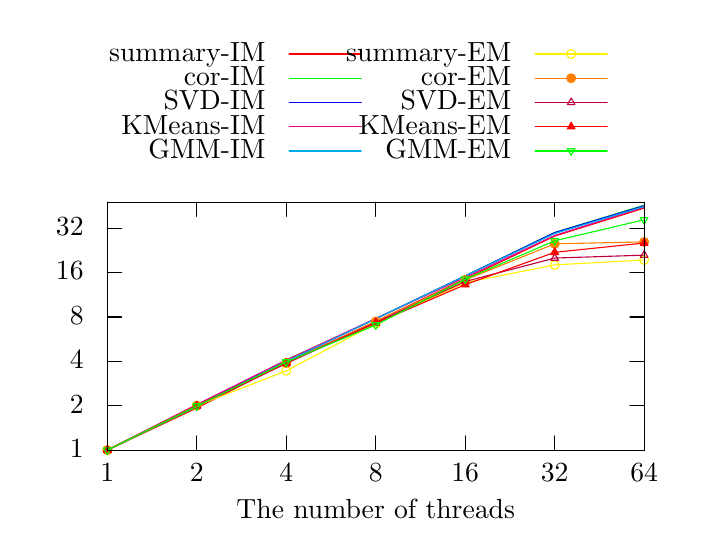
\begin{tikzpicture}[gnuplot]
%% generated with GNUPLOT 4.6p4 (Lua 5.1; terminal rev. 99, script rev. 100)
%% Wed 06 Apr 2016 02:12:53 PM EDT
\path (0.000,0.000) rectangle (8.382,6.350);
\gpcolor{color=gp lt color border}
\gpsetlinetype{gp lt border}
\gpsetlinewidth{1.00}
\draw[gp path] (1.012,0.985)--(1.192,0.985);
\draw[gp path] (7.829,0.985)--(7.649,0.985);
\node[gp node right] at (0.828,0.985) { 1};
\draw[gp path] (1.012,1.549)--(1.192,1.549);
\draw[gp path] (7.829,1.549)--(7.649,1.549);
\node[gp node right] at (0.828,1.549) { 2};
\draw[gp path] (1.012,2.112)--(1.192,2.112);
\draw[gp path] (7.829,2.112)--(7.649,2.112);
\node[gp node right] at (0.828,2.112) { 4};
\draw[gp path] (1.012,2.676)--(1.192,2.676);
\draw[gp path] (7.829,2.676)--(7.649,2.676);
\node[gp node right] at (0.828,2.676) { 8};
\draw[gp path] (1.012,3.240)--(1.192,3.240);
\draw[gp path] (7.829,3.240)--(7.649,3.240);
\node[gp node right] at (0.828,3.240) { 16};
\draw[gp path] (1.012,3.803)--(1.192,3.803);
\draw[gp path] (7.829,3.803)--(7.649,3.803);
\node[gp node right] at (0.828,3.803) { 32};
\draw[gp path] (1.012,0.985)--(1.012,1.165);
\draw[gp path] (1.012,4.133)--(1.012,3.953);
\node[gp node center] at (1.012,0.677) {1};
\draw[gp path] (2.148,0.985)--(2.148,1.165);
\draw[gp path] (2.148,4.133)--(2.148,3.953);
\node[gp node center] at (2.148,0.677) {2};
\draw[gp path] (3.284,0.985)--(3.284,1.165);
\draw[gp path] (3.284,4.133)--(3.284,3.953);
\node[gp node center] at (3.284,0.677) {4};
\draw[gp path] (4.421,0.985)--(4.421,1.165);
\draw[gp path] (4.421,4.133)--(4.421,3.953);
\node[gp node center] at (4.421,0.677) {8};
\draw[gp path] (5.557,0.985)--(5.557,1.165);
\draw[gp path] (5.557,4.133)--(5.557,3.953);
\node[gp node center] at (5.557,0.677) {16};
\draw[gp path] (6.693,0.985)--(6.693,1.165);
\draw[gp path] (6.693,4.133)--(6.693,3.953);
\node[gp node center] at (6.693,0.677) {32};
\draw[gp path] (7.829,0.985)--(7.829,1.165);
\draw[gp path] (7.829,4.133)--(7.829,3.953);
\node[gp node center] at (7.829,0.677) {64};
\draw[gp path] (1.012,4.133)--(1.012,0.985)--(7.829,0.985)--(7.829,4.133)--cycle;
\node[gp node center] at (4.420,0.215) {The number of threads};
\node[gp node right] at (3.136,6.016) {summary-IM};
\gpcolor{color=gp lt color 0}
\gpsetlinetype{gp lt plot 0}
\draw[gp path] (3.320,6.016)--(4.236,6.016);
\draw[gp path] (1.012,0.985)--(2.148,1.520)--(3.284,2.096)--(4.421,2.620)--(5.557,3.160)%
  --(6.693,3.703)--(7.829,4.058);
\gpcolor{color=gp lt color border}
\node[gp node right] at (3.136,5.708) {cor-IM};
\gpcolor{color=gp lt color 1}
\gpsetlinetype{gp lt plot 1}
\draw[gp path] (3.320,5.708)--(4.236,5.708);
\draw[gp path] (1.012,0.985)--(2.148,1.536)--(3.284,2.130)--(4.421,2.650)--(5.557,3.197)%
  --(6.693,3.749)--(7.829,4.096);
\gpcolor{color=gp lt color border}
\node[gp node right] at (3.136,5.400) {SVD-IM};
\gpcolor{color=gp lt color 2}
\gpsetlinetype{gp lt plot 2}
\draw[gp path] (3.320,5.400)--(4.236,5.400);
\draw[gp path] (1.012,0.985)--(2.148,1.557)--(3.284,2.110)--(4.421,2.655)--(5.557,3.198)%
  --(6.693,3.748)--(7.829,4.089);
\gpcolor{color=gp lt color border}
\node[gp node right] at (3.136,5.092) {KMeans-IM};
\gpcolor{color=gp lt color 3}
\gpsetlinetype{gp lt plot 3}
\draw[gp path] (3.320,5.092)--(4.236,5.092);
\draw[gp path] (1.012,0.985)--(2.148,1.565)--(3.284,2.128)--(4.421,2.657)--(5.557,3.180)%
  --(6.693,3.711)--(7.829,4.071);
\gpcolor{color=gp lt color border}
\node[gp node right] at (3.136,4.784) {GMM-IM};
\gpcolor{color=gp lt color 4}
\gpsetlinetype{gp lt plot 4}
\draw[gp path] (3.320,4.784)--(4.236,4.784);
\draw[gp path] (1.012,0.985)--(2.148,1.540)--(3.284,2.110)--(4.421,2.654)--(5.557,3.197)%
  --(6.693,3.735)--(7.829,4.078);
\gpcolor{color=gp lt color border}
\node[gp node right] at (6.260,6.016) {summary-EM};
\gpcolor{color=gp lt color 5}
\gpsetlinetype{gp lt plot 5}
\draw[gp path] (6.444,6.016)--(7.360,6.016);
\draw[gp path] (1.012,0.985)--(2.148,1.549)--(3.284,1.992)--(4.421,2.591)--(5.557,3.112)%
  --(6.693,3.337)--(7.829,3.400);
\gpsetpointsize{4.00}
\gppoint{gp mark 6}{(1.012,0.985)}
\gppoint{gp mark 6}{(2.148,1.549)}
\gppoint{gp mark 6}{(3.284,1.992)}
\gppoint{gp mark 6}{(4.421,2.591)}
\gppoint{gp mark 6}{(5.557,3.112)}
\gppoint{gp mark 6}{(6.693,3.337)}
\gppoint{gp mark 6}{(7.829,3.400)}
\gppoint{gp mark 6}{(6.902,6.016)}
\gpcolor{color=gp lt color border}
\node[gp node right] at (6.260,5.708) {cor-EM};
\gpcolor{color=gp lt color 6}
\gpsetlinetype{gp lt plot 6}
\draw[gp path] (6.444,5.708)--(7.360,5.708);
\draw[gp path] (1.012,0.985)--(2.148,1.549)--(3.284,2.092)--(4.421,2.618)--(5.557,3.147)%
  --(6.693,3.605)--(7.829,3.629);
\gppoint{gp mark 7}{(1.012,0.985)}
\gppoint{gp mark 7}{(2.148,1.549)}
\gppoint{gp mark 7}{(3.284,2.092)}
\gppoint{gp mark 7}{(4.421,2.618)}
\gppoint{gp mark 7}{(5.557,3.147)}
\gppoint{gp mark 7}{(6.693,3.605)}
\gppoint{gp mark 7}{(7.829,3.629)}
\gppoint{gp mark 7}{(6.902,5.708)}
\gpcolor{color=gp lt color border}
\node[gp node right] at (6.260,5.400) {SVD-EM};
\gpcolor{color=gp lt color 7}
\gpsetlinetype{gp lt plot 7}
\draw[gp path] (6.444,5.400)--(7.360,5.400);
\draw[gp path] (1.012,0.985)--(2.148,1.545)--(3.284,2.085)--(4.421,2.606)--(5.557,3.126)%
  --(6.693,3.424)--(7.829,3.461);
\gppoint{gp mark 8}{(1.012,0.985)}
\gppoint{gp mark 8}{(2.148,1.545)}
\gppoint{gp mark 8}{(3.284,2.085)}
\gppoint{gp mark 8}{(4.421,2.606)}
\gppoint{gp mark 8}{(5.557,3.126)}
\gppoint{gp mark 8}{(6.693,3.424)}
\gppoint{gp mark 8}{(7.829,3.461)}
\gppoint{gp mark 8}{(6.902,5.400)}
\gpcolor{color=gp lt color border}
\node[gp node right] at (6.260,5.092) {KMeans-EM};
\gpcolor{color=gp lt color 0}
\gpsetlinetype{gp lt plot 0}
\draw[gp path] (6.444,5.092)--(7.360,5.092);
\draw[gp path] (1.012,0.985)--(2.148,1.549)--(3.284,2.094)--(4.421,2.597)--(5.557,3.087)%
  --(6.693,3.497)--(7.829,3.615);
\gppoint{gp mark 9}{(1.012,0.985)}
\gppoint{gp mark 9}{(2.148,1.549)}
\gppoint{gp mark 9}{(3.284,2.094)}
\gppoint{gp mark 9}{(4.421,2.597)}
\gppoint{gp mark 9}{(5.557,3.087)}
\gppoint{gp mark 9}{(6.693,3.497)}
\gppoint{gp mark 9}{(7.829,3.615)}
\gppoint{gp mark 9}{(6.902,5.092)}
\gpcolor{color=gp lt color border}
\node[gp node right] at (6.260,4.784) {GMM-EM};
\gpcolor{color=gp lt color 1}
\gpsetlinetype{gp lt plot 1}
\draw[gp path] (6.444,4.784)--(7.360,4.784);
\draw[gp path] (1.012,0.985)--(2.148,1.545)--(3.284,2.104)--(4.421,2.574)--(5.557,3.156)%
  --(6.693,3.643)--(7.829,3.910);
\gppoint{gp mark 10}{(1.012,0.985)}
\gppoint{gp mark 10}{(2.148,1.545)}
\gppoint{gp mark 10}{(3.284,2.104)}
\gppoint{gp mark 10}{(4.421,2.574)}
\gppoint{gp mark 10}{(5.557,3.156)}
\gppoint{gp mark 10}{(6.693,3.643)}
\gppoint{gp mark 10}{(7.829,3.910)}
\gppoint{gp mark 10}{(6.902,4.784)}
\gpcolor{color=gp lt color border}
\gpsetlinetype{gp lt border}
\draw[gp path] (1.012,4.133)--(1.012,0.985)--(7.829,0.985)--(7.829,4.133)--cycle;
%% coordinates of the plot area
\gpdefrectangularnode{gp plot 1}{\pgfpoint{1.012cm}{0.985cm}}{\pgfpoint{7.829cm}{4.133cm}}
\end{tikzpicture}
%% gnuplot variables

		\vspace{-10pt}
		\caption{The speedup of FlashMatrix with multithreading both in memory (IM)
		and on SSDs (EM).}
		\label{fig:speedup}
	\end{center}
\end{figure}

The in-memory execution of FlashMatrix achieves almost linear speedup in all
applications while the out-of-core execution only
starts to flatten out after 32 threads (Figure \ref{fig:speedup}). Owing to
operation fusion in CPU cache, FlashMatrix significantly reduces data movement
between CPU and main memory. As such, memory bandwidth is no longer
the bottleneck and the computation speeds up linearly with more CPU cores
when the applications run in memory. The SSDs deliver about 10GB/s I/O throughput
and are the bottleneck for the applications with lower computation complexity.
GMM still speeds up almost linearly even when running on SSDs, due to its high
computation complexity. The performance results in Figure \ref{fig:fmR} and Figure
\ref{fig:speedup} indicate that FlashMatrix can potentially execute R code with
performance comparable to parallel C or FORTRAN implementations.

%\begin{figure}
%	\begin{center}
%		\footnotesize
%		\vspace{-15pt}
%		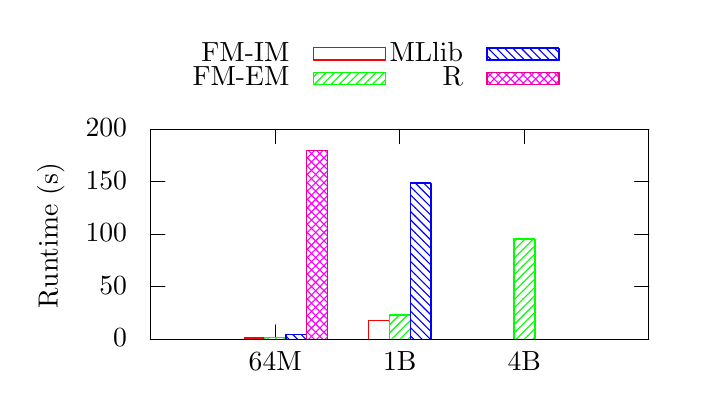
\begin{tikzpicture}[gnuplot]
%% generated with GNUPLOT 4.6p4 (Lua 5.1; terminal rev. 99, script rev. 100)
%% Fri 08 Apr 2016 08:51:15 PM EDT
\path (0.000,0.000) rectangle (8.382,4.572);
\gpcolor{color=gp lt color border}
\gpsetlinetype{gp lt border}
\gpsetlinewidth{1.00}
\draw[gp path] (1.504,0.616)--(1.684,0.616);
\draw[gp path] (7.829,0.616)--(7.649,0.616);
\node[gp node right] at (1.320,0.616) { 0};
\draw[gp path] (1.504,1.282)--(1.684,1.282);
\draw[gp path] (7.829,1.282)--(7.649,1.282);
\node[gp node right] at (1.320,1.282) { 50};
\draw[gp path] (1.504,1.948)--(1.684,1.948);
\draw[gp path] (7.829,1.948)--(7.649,1.948);
\node[gp node right] at (1.320,1.948) { 100};
\draw[gp path] (1.504,2.613)--(1.684,2.613);
\draw[gp path] (7.829,2.613)--(7.649,2.613);
\node[gp node right] at (1.320,2.613) { 150};
\draw[gp path] (1.504,3.279)--(1.684,3.279);
\draw[gp path] (7.829,3.279)--(7.649,3.279);
\node[gp node right] at (1.320,3.279) { 200};
\draw[gp path] (3.085,0.616)--(3.085,0.796);
\draw[gp path] (3.085,3.279)--(3.085,3.099);
\node[gp node center] at (3.085,0.308) {64M};
\draw[gp path] (4.667,0.616)--(4.667,0.796);
\draw[gp path] (4.667,3.279)--(4.667,3.099);
\node[gp node center] at (4.667,0.308) {1B};
\draw[gp path] (6.248,0.616)--(6.248,0.796);
\draw[gp path] (6.248,3.279)--(6.248,3.099);
\node[gp node center] at (6.248,0.308) {4B};
\draw[gp path] (1.504,3.279)--(1.504,0.616)--(7.829,0.616)--(7.829,3.279)--cycle;
\node[gp node center,rotate=-270] at (0.246,1.947) {Runtime (s)};
\node[gp node right] at (3.382,4.238) {FM-IM};
\def\gpfillpath{(3.566,4.161)--(4.482,4.161)--(4.482,4.315)--(3.566,4.315)--cycle}
\gpfill{color=gpbgfillcolor} \gpfillpath;
\gpfill{color=gp lt color 0,gp pattern 0,pattern color=.} \gpfillpath;
\gpcolor{color=gp lt color 0}
\gpsetlinetype{gp lt plot 0}
\draw[gp path] (3.566,4.161)--(4.482,4.161)--(4.482,4.315)--(3.566,4.315)--cycle;
\def\gpfillpath{(2.690,0.616)--(2.954,0.616)--(2.954,0.632)--(2.690,0.632)--cycle}
\gpfill{color=gpbgfillcolor} \gpfillpath;
\gpfill{color=gp lt color 0,gp pattern 0,pattern color=.} \gpfillpath;
\draw[gp path] (2.690,0.616)--(2.690,0.631)--(2.953,0.631)--(2.953,0.616)--cycle;
\def\gpfillpath{(4.271,0.616)--(4.536,0.616)--(4.536,0.857)--(4.271,0.857)--cycle}
\gpfill{color=gpbgfillcolor} \gpfillpath;
\gpfill{color=gp lt color 0,gp pattern 0,pattern color=.} \gpfillpath;
\draw[gp path] (4.271,0.616)--(4.271,0.856)--(4.535,0.856)--(4.535,0.616)--cycle;
\gpcolor{color=gp lt color border}
\node[gp node right] at (3.382,3.930) {FM-EM};
\def\gpfillpath{(3.566,3.853)--(4.482,3.853)--(4.482,4.007)--(3.566,4.007)--cycle}
\gpfill{color=gpbgfillcolor} \gpfillpath;
\gpfill{color=gp lt color 1,gp pattern 1,pattern color=.} \gpfillpath;
\gpcolor{color=gp lt color 1}
\gpsetlinetype{gp lt plot 1}
\draw[gp path] (3.566,3.853)--(4.482,3.853)--(4.482,4.007)--(3.566,4.007)--cycle;
\def\gpfillpath{(2.953,0.616)--(3.218,0.616)--(3.218,0.641)--(2.953,0.641)--cycle}
\gpfill{color=gpbgfillcolor} \gpfillpath;
\gpfill{color=gp lt color 1,gp pattern 1,pattern color=.} \gpfillpath;
\draw[gp path] (2.953,0.616)--(2.953,0.640)--(3.217,0.640)--(3.217,0.616)--cycle;
\def\gpfillpath{(4.535,0.616)--(4.799,0.616)--(4.799,0.928)--(4.535,0.928)--cycle}
\gpfill{color=gpbgfillcolor} \gpfillpath;
\gpfill{color=gp lt color 1,gp pattern 1,pattern color=.} \gpfillpath;
\draw[gp path] (4.535,0.616)--(4.535,0.927)--(4.798,0.927)--(4.798,0.616)--cycle;
\def\gpfillpath{(6.116,0.616)--(6.381,0.616)--(6.381,1.891)--(6.116,1.891)--cycle}
\gpfill{color=gpbgfillcolor} \gpfillpath;
\gpfill{color=gp lt color 1,gp pattern 1,pattern color=.} \gpfillpath;
\draw[gp path] (6.116,0.616)--(6.116,1.890)--(6.380,1.890)--(6.380,0.616)--cycle;
\gpcolor{color=gp lt color border}
\node[gp node right] at (5.586,4.238) {MLlib};
\def\gpfillpath{(5.770,4.161)--(6.686,4.161)--(6.686,4.315)--(5.770,4.315)--cycle}
\gpfill{color=gpbgfillcolor} \gpfillpath;
\gpfill{color=gp lt color 2,gp pattern 2,pattern color=.} \gpfillpath;
\gpcolor{color=gp lt color 2}
\gpsetlinetype{gp lt plot 2}
\draw[gp path] (5.770,4.161)--(6.686,4.161)--(6.686,4.315)--(5.770,4.315)--cycle;
\def\gpfillpath{(3.217,0.616)--(3.482,0.616)--(3.482,0.677)--(3.217,0.677)--cycle}
\gpfill{color=gpbgfillcolor} \gpfillpath;
\gpfill{color=gp lt color 2,gp pattern 2,pattern color=.} \gpfillpath;
\draw[gp path] (3.217,0.616)--(3.217,0.676)--(3.481,0.676)--(3.481,0.616)--cycle;
\def\gpfillpath{(4.798,0.616)--(5.063,0.616)--(5.063,2.601)--(4.798,2.601)--cycle}
\gpfill{color=gpbgfillcolor} \gpfillpath;
\gpfill{color=gp lt color 2,gp pattern 2,pattern color=.} \gpfillpath;
\draw[gp path] (4.798,0.616)--(4.798,2.600)--(5.062,2.600)--(5.062,0.616)--cycle;
\gpcolor{color=gp lt color border}
\node[gp node right] at (5.586,3.930) {R};
\def\gpfillpath{(5.770,3.853)--(6.686,3.853)--(6.686,4.007)--(5.770,4.007)--cycle}
\gpfill{color=gpbgfillcolor} \gpfillpath;
\gpfill{color=gp lt color 3,gp pattern 3,pattern color=.} \gpfillpath;
\gpcolor{color=gp lt color 3}
\gpsetlinetype{gp lt plot 3}
\draw[gp path] (5.770,3.853)--(6.686,3.853)--(6.686,4.007)--(5.770,4.007)--cycle;
\def\gpfillpath{(3.481,0.616)--(3.745,0.616)--(3.745,3.014)--(3.481,3.014)--cycle}
\gpfill{color=gpbgfillcolor} \gpfillpath;
\gpfill{color=gp lt color 3,gp pattern 3,pattern color=.} \gpfillpath;
\draw[gp path] (3.481,0.616)--(3.481,3.013)--(3.744,3.013)--(3.744,0.616)--cycle;
\gpcolor{color=gp lt color border}
\gpsetlinetype{gp lt border}
\draw[gp path] (1.504,3.279)--(1.504,0.616)--(7.829,0.616)--(7.829,3.279)--cycle;
%% coordinates of the plot area
\gpdefrectangularnode{gp plot 1}{\pgfpoint{1.504cm}{0.616cm}}{\pgfpoint{7.829cm}{3.279cm}}
\end{tikzpicture}
%% gnuplot variables

%		\vspace{-10pt}
%		\caption{The scalability and performance of k-means in different
%		frameworks.}
%		\label{fig:scale}
%	\end{center}
%\end{figure}

\subsection{Performance of FlashMatrix in memory and on SSDs}

We further measure the in-memory and external-memory performance of FlashMatrix
thoroughly with different datasets and
different parameters. We run the first three applications on random matrices
with the number of columns varying from 8 to 512. We run k-means
and GMM on the Friendster-32 matrix and vary the number of clusters from 2 to 64.

\begin{figure}
	\begin{center}
		\footnotesize
		\vspace{-15pt}
		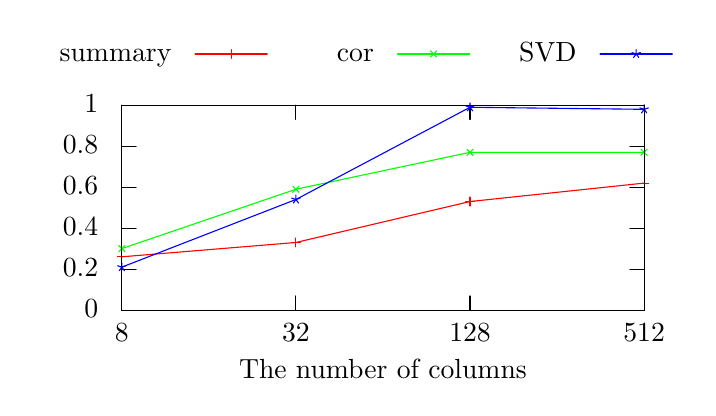
\begin{tikzpicture}[gnuplot]
%% generated with GNUPLOT 4.6p4 (Lua 5.1; terminal rev. 99, script rev. 100)
%% Sun 10 Apr 2016 09:18:38 PM EDT
\path (0.000,0.000) rectangle (8.382,4.572);
\gpcolor{color=gp lt color border}
\gpsetlinetype{gp lt border}
\gpsetlinewidth{1.00}
\draw[gp path] (1.196,0.985)--(1.376,0.985);
\draw[gp path] (7.829,0.985)--(7.649,0.985);
\node[gp node right] at (1.012,0.985) { 0};
\draw[gp path] (1.196,1.505)--(1.376,1.505);
\draw[gp path] (7.829,1.505)--(7.649,1.505);
\node[gp node right] at (1.012,1.505) { 0.2};
\draw[gp path] (1.196,2.026)--(1.376,2.026);
\draw[gp path] (7.829,2.026)--(7.649,2.026);
\node[gp node right] at (1.012,2.026) { 0.4};
\draw[gp path] (1.196,2.546)--(1.376,2.546);
\draw[gp path] (7.829,2.546)--(7.649,2.546);
\node[gp node right] at (1.012,2.546) { 0.6};
\draw[gp path] (1.196,3.067)--(1.376,3.067);
\draw[gp path] (7.829,3.067)--(7.649,3.067);
\node[gp node right] at (1.012,3.067) { 0.8};
\draw[gp path] (1.196,3.587)--(1.376,3.587);
\draw[gp path] (7.829,3.587)--(7.649,3.587);
\node[gp node right] at (1.012,3.587) { 1};
\draw[gp path] (1.196,0.985)--(1.196,1.165);
\draw[gp path] (1.196,3.587)--(1.196,3.407);
\node[gp node center] at (1.196,0.677) {8};
\draw[gp path] (3.407,0.985)--(3.407,1.165);
\draw[gp path] (3.407,3.587)--(3.407,3.407);
\node[gp node center] at (3.407,0.677) {32};
\draw[gp path] (5.618,0.985)--(5.618,1.165);
\draw[gp path] (5.618,3.587)--(5.618,3.407);
\node[gp node center] at (5.618,0.677) {128};
\draw[gp path] (7.829,0.985)--(7.829,1.165);
\draw[gp path] (7.829,3.587)--(7.829,3.407);
\node[gp node center] at (7.829,0.677) {512};
\draw[gp path] (1.196,3.587)--(1.196,0.985)--(7.829,0.985)--(7.829,3.587)--cycle;
\node[gp node center] at (4.512,0.215) {The number of columns};
\node[gp node right] at (1.942,4.238) {summary};
\gpcolor{color=gp lt color 0}
\gpsetlinetype{gp lt plot 0}
\draw[gp path] (2.126,4.238)--(3.042,4.238);
\draw[gp path] (1.196,1.662)--(3.407,1.844)--(5.618,2.364)--(7.829,2.598);
\gpsetpointsize{4.00}
\gppoint{gp mark 1}{(1.196,1.662)}
\gppoint{gp mark 1}{(3.407,1.844)}
\gppoint{gp mark 1}{(5.618,2.364)}
\gppoint{gp mark 1}{(7.829,2.598)}
\gppoint{gp mark 1}{(2.584,4.238)}
\gpcolor{color=gp lt color border}
\node[gp node right] at (4.514,4.238) {cor};
\gpcolor{color=gp lt color 1}
\gpsetlinetype{gp lt plot 1}
\draw[gp path] (4.698,4.238)--(5.614,4.238);
\draw[gp path] (1.196,1.766)--(3.407,2.520)--(5.618,2.989)--(7.829,2.989);
\gppoint{gp mark 2}{(1.196,1.766)}
\gppoint{gp mark 2}{(3.407,2.520)}
\gppoint{gp mark 2}{(5.618,2.989)}
\gppoint{gp mark 2}{(7.829,2.989)}
\gppoint{gp mark 2}{(5.156,4.238)}
\gpcolor{color=gp lt color border}
\node[gp node right] at (7.086,4.238) {SVD};
\gpcolor{color=gp lt color 2}
\gpsetlinetype{gp lt plot 2}
\draw[gp path] (7.270,4.238)--(8.186,4.238);
\draw[gp path] (1.196,1.531)--(3.407,2.390)--(5.618,3.561)--(7.829,3.535);
\gppoint{gp mark 3}{(1.196,1.531)}
\gppoint{gp mark 3}{(3.407,2.390)}
\gppoint{gp mark 3}{(5.618,3.561)}
\gppoint{gp mark 3}{(7.829,3.535)}
\gppoint{gp mark 3}{(7.728,4.238)}
\gpcolor{color=gp lt color border}
\gpsetlinetype{gp lt border}
\draw[gp path] (1.196,3.587)--(1.196,0.985)--(7.829,0.985)--(7.829,3.587)--cycle;
%% coordinates of the plot area
\gpdefrectangularnode{gp plot 1}{\pgfpoint{1.196cm}{0.985cm}}{\pgfpoint{7.829cm}{3.587cm}}
\end{tikzpicture}
%% gnuplot variables

		\vspace{-10pt}
		\caption{The relative performance of FlashMatrix on SSDs for
			statistics computation on random-65M matrices with the number of
			columns varying from 8 to 512, normalized by its performance
		in memory.}
		\label{perf:stat}
	\end{center}
\end{figure}

As the number of attributes in the datasets or the number of clusters increases,
the performance gap between in-memory and external-memory execution
narrows and eventually the external-memory performance gets almost 100\%
of in-memory performance (Figure \ref{perf:stat} and \ref{perf:clust}).
This observation conforms with the computation and I/O complexity of
the applications in Table \ref{tbl:algs}. When the number of attributes
in the dataset gets larger, the computation of matrix multiplication in
correlation and SVD grows more rapidly than I/O and eventually CPU becomes
the bottleneck. The current implementation of correlation requires an additional
pass on the input matrix to compute column-wise mean values, which results in
lower external-memory performance. Similarly,
the computation of k-means and GMM increases more rapidly than I/O and
these applications are dominated by their CPU computation as the number
of clusters gets larger. Given the I/O throughput of 10 GB/s, the applications
do not require many attributes or clusters to have their external-memory
performance close to their in-memory performance.

\begin{figure}
	\begin{center}
		\footnotesize
		\vspace{-15pt}
		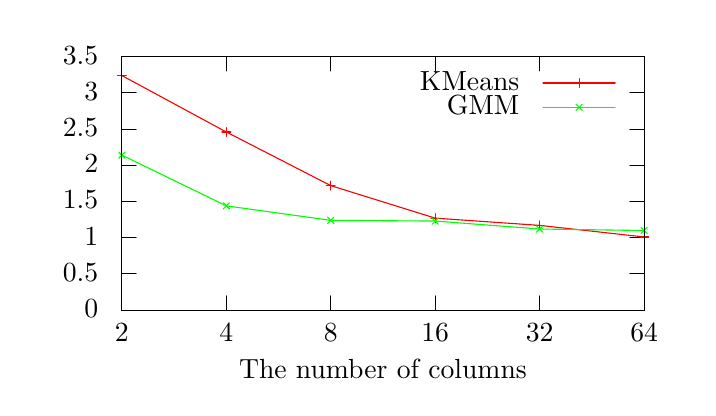
\begin{tikzpicture}[gnuplot]
%% generated with GNUPLOT 4.6p4 (Lua 5.1; terminal rev. 99, script rev. 100)
%% Wed 30 Mar 2016 08:12:03 AM EDT
\path (0.000,0.000) rectangle (8.382,4.572);
\gpcolor{color=gp lt color border}
\gpsetlinetype{gp lt border}
\gpsetlinewidth{1.00}
\draw[gp path] (1.196,0.985)--(1.376,0.985);
\draw[gp path] (7.829,0.985)--(7.649,0.985);
\node[gp node right] at (1.012,0.985) { 0};
\draw[gp path] (1.196,1.445)--(1.376,1.445);
\draw[gp path] (7.829,1.445)--(7.649,1.445);
\node[gp node right] at (1.012,1.445) { 0.5};
\draw[gp path] (1.196,1.904)--(1.376,1.904);
\draw[gp path] (7.829,1.904)--(7.649,1.904);
\node[gp node right] at (1.012,1.904) { 1};
\draw[gp path] (1.196,2.364)--(1.376,2.364);
\draw[gp path] (7.829,2.364)--(7.649,2.364);
\node[gp node right] at (1.012,2.364) { 1.5};
\draw[gp path] (1.196,2.824)--(1.376,2.824);
\draw[gp path] (7.829,2.824)--(7.649,2.824);
\node[gp node right] at (1.012,2.824) { 2};
\draw[gp path] (1.196,3.284)--(1.376,3.284);
\draw[gp path] (7.829,3.284)--(7.649,3.284);
\node[gp node right] at (1.012,3.284) { 2.5};
\draw[gp path] (1.196,3.743)--(1.376,3.743);
\draw[gp path] (7.829,3.743)--(7.649,3.743);
\node[gp node right] at (1.012,3.743) { 3};
\draw[gp path] (1.196,4.203)--(1.376,4.203);
\draw[gp path] (7.829,4.203)--(7.649,4.203);
\node[gp node right] at (1.012,4.203) { 3.5};
\draw[gp path] (1.196,0.985)--(1.196,1.165);
\draw[gp path] (1.196,4.203)--(1.196,4.023);
\node[gp node center] at (1.196,0.677) {2};
\draw[gp path] (2.523,0.985)--(2.523,1.165);
\draw[gp path] (2.523,4.203)--(2.523,4.023);
\node[gp node center] at (2.523,0.677) {4};
\draw[gp path] (3.849,0.985)--(3.849,1.165);
\draw[gp path] (3.849,4.203)--(3.849,4.023);
\node[gp node center] at (3.849,0.677) {8};
\draw[gp path] (5.176,0.985)--(5.176,1.165);
\draw[gp path] (5.176,4.203)--(5.176,4.023);
\node[gp node center] at (5.176,0.677) {16};
\draw[gp path] (6.502,0.985)--(6.502,1.165);
\draw[gp path] (6.502,4.203)--(6.502,4.023);
\node[gp node center] at (6.502,0.677) {32};
\draw[gp path] (7.829,0.985)--(7.829,1.165);
\draw[gp path] (7.829,4.203)--(7.829,4.023);
\node[gp node center] at (7.829,0.677) {64};
\draw[gp path] (1.196,4.203)--(1.196,0.985)--(7.829,0.985)--(7.829,4.203)--cycle;
\node[gp node center] at (4.512,0.215) {The number of columns};
\node[gp node right] at (6.361,3.869) {KMeans};
\gpcolor{color=gp lt color 0}
\gpsetlinetype{gp lt plot 0}
\draw[gp path] (6.545,3.869)--(7.461,3.869);
\draw[gp path] (1.196,3.964)--(2.523,3.247)--(3.849,2.566)--(5.176,2.153)--(6.502,2.061)%
  --(7.829,1.914);
\gpsetpointsize{4.00}
\gppoint{gp mark 1}{(1.196,3.964)}
\gppoint{gp mark 1}{(2.523,3.247)}
\gppoint{gp mark 1}{(3.849,2.566)}
\gppoint{gp mark 1}{(5.176,2.153)}
\gppoint{gp mark 1}{(6.502,2.061)}
\gppoint{gp mark 1}{(7.829,1.914)}
\gppoint{gp mark 1}{(7.003,3.869)}
\gpcolor{color=gp lt color border}
\node[gp node right] at (6.361,3.561) {GMM};
\gpcolor{color=gp lt color 1}
\gpsetlinetype{gp lt plot 1}
\draw[gp path] (6.545,3.561)--(7.461,3.561);
\draw[gp path] (1.196,2.953)--(2.523,2.309)--(3.849,2.125)--(5.176,2.116)--(6.502,2.015)%
  --(7.829,1.996);
\gppoint{gp mark 2}{(1.196,2.953)}
\gppoint{gp mark 2}{(2.523,2.309)}
\gppoint{gp mark 2}{(3.849,2.125)}
\gppoint{gp mark 2}{(5.176,2.116)}
\gppoint{gp mark 2}{(6.502,2.015)}
\gppoint{gp mark 2}{(7.829,1.996)}
\gppoint{gp mark 2}{(7.003,3.561)}
\gpcolor{color=gp lt color border}
\gpsetlinetype{gp lt border}
\draw[gp path] (1.196,4.203)--(1.196,0.985)--(7.829,0.985)--(7.829,4.203)--cycle;
%% coordinates of the plot area
\gpdefrectangularnode{gp plot 1}{\pgfpoint{1.196cm}{0.985cm}}{\pgfpoint{7.829cm}{4.203cm}}
\end{tikzpicture}
%% gnuplot variables

		\vspace{-10pt}
		\caption{The relative performance of FlashMatrix on SSDs for
			clustering algorithms with different numbers of clusters, normalized
		by its performance in memory.}
		\label{perf:clust}
	\end{center}
\end{figure}

\subsection{Effectiveness of optimizations}

In this section, we illustrate the effectiveness of our memory and CPU
optimizations in FlashMatrix. To reduce memory overhead, we focus on three
main optimizations: \textit{(i)} reusing memory chunks for new in-memory
matrices and I/O access to reduce large
memory allocation, \textit{(ii)} matrix operation fusion in main
memory to reduce data movement between SSDs and main memory, \textit{(iii)}
matrix operation fusion in CPU cache to reduce data movement between main
memory and CPU cache. To reduce computation overhead, we illustrate
the effectiveness of using VUDFs.

Each memory optimization has significant performance improvement on most of
the applications when they are executed on SSDs (Figure \ref{perf:opts}).
Due to the space limit, we only illustrate the effectiveness of the memory
optimizations in out-of-core execution. Operation fusion in main memory achieves
the highest performance improvement in almost all applications, even in GMM,
which has the highest asymptotic computation complexity. Even though the SSDs
deliver 10GB/s I/O throughput, materializing every matrix operation separately
causes SSDs to be the main bottleneck in the system.
Fusing matrix operations in memory significantly reduces the burden on SSDs and
improves performance by a large factor. Operation fusion in the CPU cache also
has very positive performance impact on some applications even when
the applications run on SSDs. This suggests that with sufficient I/O optimizations,
many machine learning applications that run on fast SSDs can be bottlenecked by
the bandwidth of main memory, instead of I/O. Even though it is less noticeable,
reducing large memory allocation improves I/O performance and almost doubles
the overall performance of all applications.

\begin{figure}
	\begin{center}
		\footnotesize
		\vspace{-15pt}
		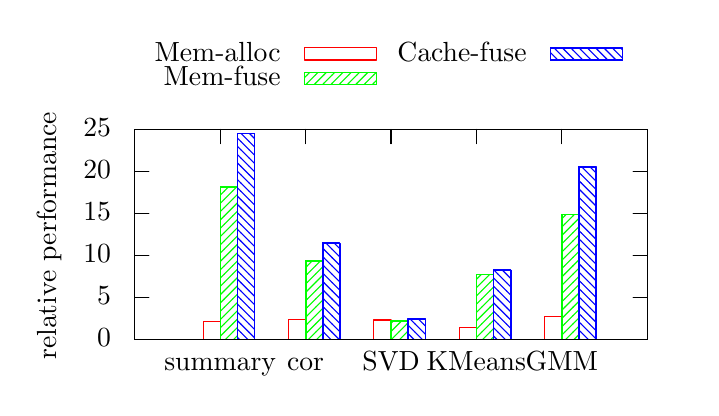
\begin{tikzpicture}[gnuplot]
%% generated with GNUPLOT 4.6p4 (Lua 5.1; terminal rev. 99, script rev. 100)
%% Mon 04 Apr 2016 04:07:38 PM EDT
\path (0.000,0.000) rectangle (8.382,4.572);
\gpcolor{color=gp lt color border}
\gpsetlinetype{gp lt border}
\gpsetlinewidth{1.00}
\draw[gp path] (1.320,0.616)--(1.500,0.616);
\draw[gp path] (7.829,0.616)--(7.649,0.616);
\node[gp node right] at (1.136,0.616) { 0};
\draw[gp path] (1.320,1.149)--(1.500,1.149);
\draw[gp path] (7.829,1.149)--(7.649,1.149);
\node[gp node right] at (1.136,1.149) { 5};
\draw[gp path] (1.320,1.681)--(1.500,1.681);
\draw[gp path] (7.829,1.681)--(7.649,1.681);
\node[gp node right] at (1.136,1.681) { 10};
\draw[gp path] (1.320,2.214)--(1.500,2.214);
\draw[gp path] (7.829,2.214)--(7.649,2.214);
\node[gp node right] at (1.136,2.214) { 15};
\draw[gp path] (1.320,2.746)--(1.500,2.746);
\draw[gp path] (7.829,2.746)--(7.649,2.746);
\node[gp node right] at (1.136,2.746) { 20};
\draw[gp path] (1.320,3.279)--(1.500,3.279);
\draw[gp path] (7.829,3.279)--(7.649,3.279);
\node[gp node right] at (1.136,3.279) { 25};
\draw[gp path] (2.405,0.616)--(2.405,0.796);
\draw[gp path] (2.405,3.279)--(2.405,3.099);
\node[gp node center] at (2.405,0.308) {summary};
\draw[gp path] (3.490,0.616)--(3.490,0.796);
\draw[gp path] (3.490,3.279)--(3.490,3.099);
\node[gp node center] at (3.490,0.308) {cor};
\draw[gp path] (4.575,0.616)--(4.575,0.796);
\draw[gp path] (4.575,3.279)--(4.575,3.099);
\node[gp node center] at (4.575,0.308) {SVD};
\draw[gp path] (5.659,0.616)--(5.659,0.796);
\draw[gp path] (5.659,3.279)--(5.659,3.099);
\node[gp node center] at (5.659,0.308) {KMeans};
\draw[gp path] (6.744,0.616)--(6.744,0.796);
\draw[gp path] (6.744,3.279)--(6.744,3.099);
\node[gp node center] at (6.744,0.308) {GMM};
\draw[gp path] (1.320,3.279)--(1.320,0.616)--(7.829,0.616)--(7.829,3.279)--cycle;
\node[gp node center,rotate=-270] at (0.246,1.947) {relative performance};
\node[gp node right] at (3.290,4.238) {Mem-alloc};
\def\gpfillpath{(3.474,4.161)--(4.390,4.161)--(4.390,4.315)--(3.474,4.315)--cycle}
\gpfill{color=gpbgfillcolor} \gpfillpath;
\gpfill{color=gp lt color 0,gp pattern 0,pattern color=.} \gpfillpath;
\gpcolor{color=gp lt color 0}
\gpsetlinetype{gp lt plot 0}
\draw[gp path] (3.474,4.161)--(4.390,4.161)--(4.390,4.315)--(3.474,4.315)--cycle;
\def\gpfillpath{(2.188,0.616)--(2.406,0.616)--(2.406,0.844)--(2.188,0.844)--cycle}
\gpfill{color=gpbgfillcolor} \gpfillpath;
\gpfill{color=gp lt color 0,gp pattern 0,pattern color=.} \gpfillpath;
\draw[gp path] (2.188,0.616)--(2.188,0.843)--(2.405,0.843)--(2.405,0.616)--cycle;
\def\gpfillpath{(3.273,0.616)--(3.491,0.616)--(3.491,0.872)--(3.273,0.872)--cycle}
\gpfill{color=gpbgfillcolor} \gpfillpath;
\gpfill{color=gp lt color 0,gp pattern 0,pattern color=.} \gpfillpath;
\draw[gp path] (3.273,0.616)--(3.273,0.871)--(3.490,0.871)--(3.490,0.616)--cycle;
\def\gpfillpath{(4.358,0.616)--(4.576,0.616)--(4.576,0.861)--(4.358,0.861)--cycle}
\gpfill{color=gpbgfillcolor} \gpfillpath;
\gpfill{color=gp lt color 0,gp pattern 0,pattern color=.} \gpfillpath;
\draw[gp path] (4.358,0.616)--(4.358,0.860)--(4.575,0.860)--(4.575,0.616)--cycle;
\def\gpfillpath{(5.442,0.616)--(5.660,0.616)--(5.660,0.764)--(5.442,0.764)--cycle}
\gpfill{color=gpbgfillcolor} \gpfillpath;
\gpfill{color=gp lt color 0,gp pattern 0,pattern color=.} \gpfillpath;
\draw[gp path] (5.442,0.616)--(5.442,0.763)--(5.659,0.763)--(5.659,0.616)--cycle;
\def\gpfillpath{(6.527,0.616)--(6.745,0.616)--(6.745,0.908)--(6.527,0.908)--cycle}
\gpfill{color=gpbgfillcolor} \gpfillpath;
\gpfill{color=gp lt color 0,gp pattern 0,pattern color=.} \gpfillpath;
\draw[gp path] (6.527,0.616)--(6.527,0.907)--(6.744,0.907)--(6.744,0.616)--cycle;
\gpcolor{color=gp lt color border}
\node[gp node right] at (3.290,3.930) {Mem-fuse};
\def\gpfillpath{(3.474,3.853)--(4.390,3.853)--(4.390,4.007)--(3.474,4.007)--cycle}
\gpfill{color=gpbgfillcolor} \gpfillpath;
\gpfill{color=gp lt color 1,gp pattern 1,pattern color=.} \gpfillpath;
\gpcolor{color=gp lt color 1}
\gpsetlinetype{gp lt plot 1}
\draw[gp path] (3.474,3.853)--(4.390,3.853)--(4.390,4.007)--(3.474,4.007)--cycle;
\def\gpfillpath{(2.405,0.616)--(2.623,0.616)--(2.623,2.554)--(2.405,2.554)--cycle}
\gpfill{color=gpbgfillcolor} \gpfillpath;
\gpfill{color=gp lt color 1,gp pattern 1,pattern color=.} \gpfillpath;
\draw[gp path] (2.405,0.616)--(2.405,2.553)--(2.622,2.553)--(2.622,0.616)--cycle;
\def\gpfillpath{(3.490,0.616)--(3.708,0.616)--(3.708,1.611)--(3.490,1.611)--cycle}
\gpfill{color=gpbgfillcolor} \gpfillpath;
\gpfill{color=gp lt color 1,gp pattern 1,pattern color=.} \gpfillpath;
\draw[gp path] (3.490,0.616)--(3.490,1.610)--(3.707,1.610)--(3.707,0.616)--cycle;
\def\gpfillpath{(4.575,0.616)--(4.792,0.616)--(4.792,0.852)--(4.575,0.852)--cycle}
\gpfill{color=gpbgfillcolor} \gpfillpath;
\gpfill{color=gp lt color 1,gp pattern 1,pattern color=.} \gpfillpath;
\draw[gp path] (4.575,0.616)--(4.575,0.851)--(4.791,0.851)--(4.791,0.616)--cycle;
\def\gpfillpath{(5.659,0.616)--(5.877,0.616)--(5.877,1.437)--(5.659,1.437)--cycle}
\gpfill{color=gpbgfillcolor} \gpfillpath;
\gpfill{color=gp lt color 1,gp pattern 1,pattern color=.} \gpfillpath;
\draw[gp path] (5.659,0.616)--(5.659,1.436)--(5.876,1.436)--(5.876,0.616)--cycle;
\def\gpfillpath{(6.744,0.616)--(6.962,0.616)--(6.962,2.204)--(6.744,2.204)--cycle}
\gpfill{color=gpbgfillcolor} \gpfillpath;
\gpfill{color=gp lt color 1,gp pattern 1,pattern color=.} \gpfillpath;
\draw[gp path] (6.744,0.616)--(6.744,2.203)--(6.961,2.203)--(6.961,0.616)--cycle;
\gpcolor{color=gp lt color border}
\node[gp node right] at (6.414,4.238) {Cache-fuse};
\def\gpfillpath{(6.598,4.161)--(7.514,4.161)--(7.514,4.315)--(6.598,4.315)--cycle}
\gpfill{color=gpbgfillcolor} \gpfillpath;
\gpfill{color=gp lt color 2,gp pattern 2,pattern color=.} \gpfillpath;
\gpcolor{color=gp lt color 2}
\gpsetlinetype{gp lt plot 2}
\draw[gp path] (6.598,4.161)--(7.514,4.161)--(7.514,4.315)--(6.598,4.315)--cycle;
\def\gpfillpath{(2.622,0.616)--(2.840,0.616)--(2.840,3.230)--(2.622,3.230)--cycle}
\gpfill{color=gpbgfillcolor} \gpfillpath;
\gpfill{color=gp lt color 2,gp pattern 2,pattern color=.} \gpfillpath;
\draw[gp path] (2.622,0.616)--(2.622,3.229)--(2.839,3.229)--(2.839,0.616)--cycle;
\def\gpfillpath{(3.707,0.616)--(3.925,0.616)--(3.925,1.842)--(3.707,1.842)--cycle}
\gpfill{color=gpbgfillcolor} \gpfillpath;
\gpfill{color=gp lt color 2,gp pattern 2,pattern color=.} \gpfillpath;
\draw[gp path] (3.707,0.616)--(3.707,1.841)--(3.924,1.841)--(3.924,0.616)--cycle;
\def\gpfillpath{(4.791,0.616)--(5.009,0.616)--(5.009,0.876)--(4.791,0.876)--cycle}
\gpfill{color=gpbgfillcolor} \gpfillpath;
\gpfill{color=gp lt color 2,gp pattern 2,pattern color=.} \gpfillpath;
\draw[gp path] (4.791,0.616)--(4.791,0.875)--(5.008,0.875)--(5.008,0.616)--cycle;
\def\gpfillpath{(5.876,0.616)--(6.094,0.616)--(6.094,1.499)--(5.876,1.499)--cycle}
\gpfill{color=gpbgfillcolor} \gpfillpath;
\gpfill{color=gp lt color 2,gp pattern 2,pattern color=.} \gpfillpath;
\draw[gp path] (5.876,0.616)--(5.876,1.498)--(6.093,1.498)--(6.093,0.616)--cycle;
\def\gpfillpath{(6.961,0.616)--(7.179,0.616)--(7.179,2.807)--(6.961,2.807)--cycle}
\gpfill{color=gpbgfillcolor} \gpfillpath;
\gpfill{color=gp lt color 2,gp pattern 2,pattern color=.} \gpfillpath;
\draw[gp path] (6.961,0.616)--(6.961,2.806)--(7.178,2.806)--(7.178,0.616)--cycle;
\gpcolor{color=gp lt color border}
\gpsetlinetype{gp lt border}
\draw[gp path] (1.320,3.279)--(1.320,0.616)--(7.829,0.616)--(7.829,3.279)--cycle;
%% coordinates of the plot area
\gpdefrectangularnode{gp plot 1}{\pgfpoint{1.320cm}{0.616cm}}{\pgfpoint{7.829cm}{3.279cm}}
\end{tikzpicture}
%% gnuplot variables

		\vspace{-10pt}
		\caption{The effectiveness of memory optimizations on different
			applications when they are executed on SSDs. The three memory
		optimizations are applied to FlashMatrix incrementally.}
		\label{perf:opts}
	\end{center}
\end{figure}

Using VUDFs improves the performance of the applications that rely on GenOps
for computation (Figure \ref{perf:opts_CPU}). In this experiment, the base
implementations deploy all memory optimizations to avoid memory from being
the bottleneck of the system,
and invoke functions on individual elements in
matrices. The FlashMatrix implementations of computing statistical summary
and k-means solely rely on GenOps. Therefore, their performance is almost doubled
when using VUDFs. The main computation in correlation and GMM is matrix
multiplication, but they still rely on GenOps for the remaining computation.
As such, using VUDFs help their performance. SVD solely uses matrix
multiplication, so switching VUDFs has no performance impact.

\begin{figure}
	\begin{center}
		\footnotesize
		\vspace{-15pt}
		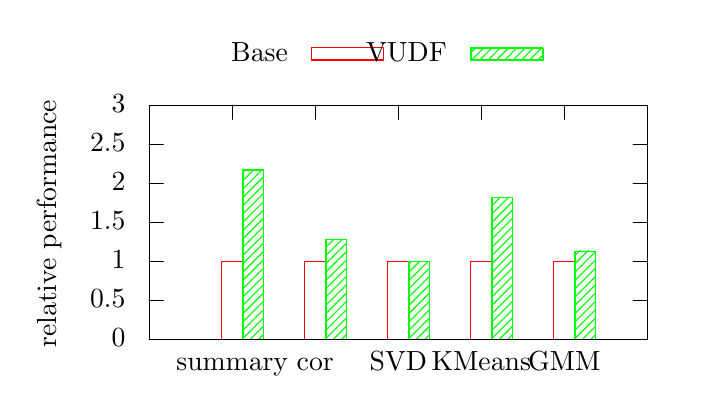
\begin{tikzpicture}[gnuplot]
%% generated with GNUPLOT 4.6p4 (Lua 5.1; terminal rev. 99, script rev. 100)
%% Sat 09 Apr 2016 04:07:24 PM EDT
\path (0.000,0.000) rectangle (8.382,4.572);
\gpcolor{color=gp lt color border}
\gpsetlinetype{gp lt border}
\gpsetlinewidth{1.00}
\draw[gp path] (1.504,0.616)--(1.684,0.616);
\draw[gp path] (7.829,0.616)--(7.649,0.616);
\node[gp node right] at (1.320,0.616) { 0};
\draw[gp path] (1.504,1.111)--(1.684,1.111);
\draw[gp path] (7.829,1.111)--(7.649,1.111);
\node[gp node right] at (1.320,1.111) { 0.5};
\draw[gp path] (1.504,1.606)--(1.684,1.606);
\draw[gp path] (7.829,1.606)--(7.649,1.606);
\node[gp node right] at (1.320,1.606) { 1};
\draw[gp path] (1.504,2.102)--(1.684,2.102);
\draw[gp path] (7.829,2.102)--(7.649,2.102);
\node[gp node right] at (1.320,2.102) { 1.5};
\draw[gp path] (1.504,2.597)--(1.684,2.597);
\draw[gp path] (7.829,2.597)--(7.649,2.597);
\node[gp node right] at (1.320,2.597) { 2};
\draw[gp path] (1.504,3.092)--(1.684,3.092);
\draw[gp path] (7.829,3.092)--(7.649,3.092);
\node[gp node right] at (1.320,3.092) { 2.5};
\draw[gp path] (1.504,3.587)--(1.684,3.587);
\draw[gp path] (7.829,3.587)--(7.649,3.587);
\node[gp node right] at (1.320,3.587) { 3};
\draw[gp path] (2.558,0.616)--(2.558,0.796);
\draw[gp path] (2.558,3.587)--(2.558,3.407);
\node[gp node center] at (2.558,0.308) {summary};
\draw[gp path] (3.612,0.616)--(3.612,0.796);
\draw[gp path] (3.612,3.587)--(3.612,3.407);
\node[gp node center] at (3.612,0.308) {cor};
\draw[gp path] (4.667,0.616)--(4.667,0.796);
\draw[gp path] (4.667,3.587)--(4.667,3.407);
\node[gp node center] at (4.667,0.308) {SVD};
\draw[gp path] (5.721,0.616)--(5.721,0.796);
\draw[gp path] (5.721,3.587)--(5.721,3.407);
\node[gp node center] at (5.721,0.308) {KMeans};
\draw[gp path] (6.775,0.616)--(6.775,0.796);
\draw[gp path] (6.775,3.587)--(6.775,3.407);
\node[gp node center] at (6.775,0.308) {GMM};
\draw[gp path] (1.504,3.587)--(1.504,0.616)--(7.829,0.616)--(7.829,3.587)--cycle;
\node[gp node center,rotate=-270] at (0.246,2.101) {relative performance};
\node[gp node right] at (3.382,4.238) {Base};
\def\gpfillpath{(3.566,4.161)--(4.482,4.161)--(4.482,4.315)--(3.566,4.315)--cycle}
\gpfill{color=gpbgfillcolor} \gpfillpath;
\gpfill{color=gp lt color 0,gp pattern 0,pattern color=.} \gpfillpath;
\gpcolor{color=gp lt color 0}
\gpsetlinetype{gp lt plot 0}
\draw[gp path] (3.566,4.161)--(4.482,4.161)--(4.482,4.315)--(3.566,4.315)--cycle;
\def\gpfillpath{(2.426,0.616)--(2.691,0.616)--(2.691,1.607)--(2.426,1.607)--cycle}
\gpfill{color=gpbgfillcolor} \gpfillpath;
\gpfill{color=gp lt color 0,gp pattern 0,pattern color=.} \gpfillpath;
\draw[gp path] (2.426,0.616)--(2.426,1.606)--(2.690,1.606)--(2.690,0.616)--cycle;
\def\gpfillpath{(3.481,0.616)--(3.745,0.616)--(3.745,1.607)--(3.481,1.607)--cycle}
\gpfill{color=gpbgfillcolor} \gpfillpath;
\gpfill{color=gp lt color 0,gp pattern 0,pattern color=.} \gpfillpath;
\draw[gp path] (3.481,0.616)--(3.481,1.606)--(3.744,1.606)--(3.744,0.616)--cycle;
\def\gpfillpath{(4.535,0.616)--(4.799,0.616)--(4.799,1.607)--(4.535,1.607)--cycle}
\gpfill{color=gpbgfillcolor} \gpfillpath;
\gpfill{color=gp lt color 0,gp pattern 0,pattern color=.} \gpfillpath;
\draw[gp path] (4.535,0.616)--(4.535,1.606)--(4.798,1.606)--(4.798,0.616)--cycle;
\def\gpfillpath{(5.589,0.616)--(5.853,0.616)--(5.853,1.607)--(5.589,1.607)--cycle}
\gpfill{color=gpbgfillcolor} \gpfillpath;
\gpfill{color=gp lt color 0,gp pattern 0,pattern color=.} \gpfillpath;
\draw[gp path] (5.589,0.616)--(5.589,1.606)--(5.852,1.606)--(5.852,0.616)--cycle;
\def\gpfillpath{(6.643,0.616)--(6.908,0.616)--(6.908,1.607)--(6.643,1.607)--cycle}
\gpfill{color=gpbgfillcolor} \gpfillpath;
\gpfill{color=gp lt color 0,gp pattern 0,pattern color=.} \gpfillpath;
\draw[gp path] (6.643,0.616)--(6.643,1.606)--(6.907,1.606)--(6.907,0.616)--cycle;
\gpcolor{color=gp lt color border}
\node[gp node right] at (5.402,4.238) {VUDF};
\def\gpfillpath{(5.586,4.161)--(6.502,4.161)--(6.502,4.315)--(5.586,4.315)--cycle}
\gpfill{color=gpbgfillcolor} \gpfillpath;
\gpfill{color=gp lt color 1,gp pattern 1,pattern color=.} \gpfillpath;
\gpcolor{color=gp lt color 1}
\gpsetlinetype{gp lt plot 1}
\draw[gp path] (5.586,4.161)--(6.502,4.161)--(6.502,4.315)--(5.586,4.315)--cycle;
\def\gpfillpath{(2.690,0.616)--(2.954,0.616)--(2.954,2.766)--(2.690,2.766)--cycle}
\gpfill{color=gpbgfillcolor} \gpfillpath;
\gpfill{color=gp lt color 1,gp pattern 1,pattern color=.} \gpfillpath;
\draw[gp path] (2.690,0.616)--(2.690,2.765)--(2.953,2.765)--(2.953,0.616)--cycle;
\def\gpfillpath{(3.744,0.616)--(4.009,0.616)--(4.009,1.885)--(3.744,1.885)--cycle}
\gpfill{color=gpbgfillcolor} \gpfillpath;
\gpfill{color=gp lt color 1,gp pattern 1,pattern color=.} \gpfillpath;
\draw[gp path] (3.744,0.616)--(3.744,1.884)--(4.008,1.884)--(4.008,0.616)--cycle;
\def\gpfillpath{(4.798,0.616)--(5.063,0.616)--(5.063,1.607)--(4.798,1.607)--cycle}
\gpfill{color=gpbgfillcolor} \gpfillpath;
\gpfill{color=gp lt color 1,gp pattern 1,pattern color=.} \gpfillpath;
\draw[gp path] (4.798,0.616)--(4.798,1.606)--(5.062,1.606)--(5.062,0.616)--cycle;
\def\gpfillpath{(5.852,0.616)--(6.117,0.616)--(6.117,2.419)--(5.852,2.419)--cycle}
\gpfill{color=gpbgfillcolor} \gpfillpath;
\gpfill{color=gp lt color 1,gp pattern 1,pattern color=.} \gpfillpath;
\draw[gp path] (5.852,0.616)--(5.852,2.418)--(6.116,2.418)--(6.116,0.616)--cycle;
\def\gpfillpath{(6.907,0.616)--(7.171,0.616)--(7.171,1.736)--(6.907,1.736)--cycle}
\gpfill{color=gpbgfillcolor} \gpfillpath;
\gpfill{color=gp lt color 1,gp pattern 1,pattern color=.} \gpfillpath;
\draw[gp path] (6.907,0.616)--(6.907,1.735)--(7.170,1.735)--(7.170,0.616)--cycle;
\gpcolor{color=gp lt color border}
\gpsetlinetype{gp lt border}
\draw[gp path] (1.504,3.587)--(1.504,0.616)--(7.829,0.616)--(7.829,3.587)--cycle;
%% coordinates of the plot area
\gpdefrectangularnode{gp plot 1}{\pgfpoint{1.504cm}{0.616cm}}{\pgfpoint{7.829cm}{3.587cm}}
\end{tikzpicture}
%% gnuplot variables

		\vspace{-10pt}
		\caption{The effectiveness of using VUDFs on different applications
		when they are executed in memory.}
		\label{perf:opts_CPU}
	\end{center}
\end{figure}


\section{Conclusions}
We present FlashR, a matrix-oriented programming framework that executes
R-programmed machine learning algorithms in parallel and out-of-core
automatically. FlashR scales to large datasets by utilizing commodity SSDs.

%For simplicity and generality, the core of FlashR only implements
%a small number of generalized matrix operators (GenOps). It reimplements
%many matrix operations in R \textit{base} package with GenOps to provide
%a familiar programming environment to users. To improve performance,
%FlashR uses vectorized element functions (VEleFuns) to reduce the
%overhead of function calls and fuses matrix operations to reduce data movement
%between CPU and SSDs.

Although R is considered to be slow and unable to scale to large datasets,
we demonstrate that with sufficient system-level optimizations, FlashR powers
the R programming interface to achieve high performance and scalability
for developing many machine learning algorithms. R implementations executed in FlashR
outperform H$_2$O and Spark MLlib on all algorithms by a factor of $3-20$, using
the same shared memory hardware. FlashR scales to datasets with billions of
data points easily with negligible amounts of memory and completes all
algorithms within a reasonable amount of time.

Even though the current I/O technologies, such as solid-state drives (SSDs),
are an order of magnitude slower than DRAM, the external-memory execution
of many algorithms in FlashR achieves performance approaching their in-memory
execution. We demonstrate that an I/O throughput of 10 GB/s saturates the CPU
for many algorithms, even in a large parallel NUMA machine. 

FlashR simplifies the programming effort of writing parallel and out-of-core
implementations for large-scale machine learning. With FlashR, machine learning
researchers can prototype algorithms in a familiar programming environment,
while still getting efficient and scalable implementations.
We believe FlashR provides new opportunities for developing large-scale
machine learning algorithms.


%\section{Acknowledgments}


{\footnotesize \bibliographystyle{acm}
\bibliography{FlashMatrix}  % sigproc.bib is the name of the Bibliography in this case


%\theendnotes

\end{document}
